% Options for packages loaded elsewhere
% Options for packages loaded elsewhere
\PassOptionsToPackage{unicode}{hyperref}
\PassOptionsToPackage{hyphens}{url}
\PassOptionsToPackage{dvipsnames,svgnames,x11names}{xcolor}
%
\documentclass[
  letterpaper,
  DIV=11,
  numbers=noendperiod]{scrartcl}
\usepackage{xcolor}
\usepackage{amsmath,amssymb}
\setcounter{secnumdepth}{-\maxdimen} % remove section numbering
\usepackage{iftex}
\ifPDFTeX
  \usepackage[T1]{fontenc}
  \usepackage[utf8]{inputenc}
  \usepackage{textcomp} % provide euro and other symbols
\else % if luatex or xetex
  \usepackage{unicode-math} % this also loads fontspec
  \defaultfontfeatures{Scale=MatchLowercase}
  \defaultfontfeatures[\rmfamily]{Ligatures=TeX,Scale=1}
\fi
\usepackage{lmodern}
\ifPDFTeX\else
  % xetex/luatex font selection
\fi
% Use upquote if available, for straight quotes in verbatim environments
\IfFileExists{upquote.sty}{\usepackage{upquote}}{}
\IfFileExists{microtype.sty}{% use microtype if available
  \usepackage[]{microtype}
  \UseMicrotypeSet[protrusion]{basicmath} % disable protrusion for tt fonts
}{}
\makeatletter
\@ifundefined{KOMAClassName}{% if non-KOMA class
  \IfFileExists{parskip.sty}{%
    \usepackage{parskip}
  }{% else
    \setlength{\parindent}{0pt}
    \setlength{\parskip}{6pt plus 2pt minus 1pt}}
}{% if KOMA class
  \KOMAoptions{parskip=half}}
\makeatother
% Make \paragraph and \subparagraph free-standing
\makeatletter
\ifx\paragraph\undefined\else
  \let\oldparagraph\paragraph
  \renewcommand{\paragraph}{
    \@ifstar
      \xxxParagraphStar
      \xxxParagraphNoStar
  }
  \newcommand{\xxxParagraphStar}[1]{\oldparagraph*{#1}\mbox{}}
  \newcommand{\xxxParagraphNoStar}[1]{\oldparagraph{#1}\mbox{}}
\fi
\ifx\subparagraph\undefined\else
  \let\oldsubparagraph\subparagraph
  \renewcommand{\subparagraph}{
    \@ifstar
      \xxxSubParagraphStar
      \xxxSubParagraphNoStar
  }
  \newcommand{\xxxSubParagraphStar}[1]{\oldsubparagraph*{#1}\mbox{}}
  \newcommand{\xxxSubParagraphNoStar}[1]{\oldsubparagraph{#1}\mbox{}}
\fi
\makeatother

\usepackage{color}
\usepackage{fancyvrb}
\newcommand{\VerbBar}{|}
\newcommand{\VERB}{\Verb[commandchars=\\\{\}]}
\DefineVerbatimEnvironment{Highlighting}{Verbatim}{commandchars=\\\{\}}
% Add ',fontsize=\small' for more characters per line
\usepackage{framed}
\definecolor{shadecolor}{RGB}{241,243,245}
\newenvironment{Shaded}{\begin{snugshade}}{\end{snugshade}}
\newcommand{\AlertTok}[1]{\textcolor[rgb]{0.68,0.00,0.00}{#1}}
\newcommand{\AnnotationTok}[1]{\textcolor[rgb]{0.37,0.37,0.37}{#1}}
\newcommand{\AttributeTok}[1]{\textcolor[rgb]{0.40,0.45,0.13}{#1}}
\newcommand{\BaseNTok}[1]{\textcolor[rgb]{0.68,0.00,0.00}{#1}}
\newcommand{\BuiltInTok}[1]{\textcolor[rgb]{0.00,0.23,0.31}{#1}}
\newcommand{\CharTok}[1]{\textcolor[rgb]{0.13,0.47,0.30}{#1}}
\newcommand{\CommentTok}[1]{\textcolor[rgb]{0.37,0.37,0.37}{#1}}
\newcommand{\CommentVarTok}[1]{\textcolor[rgb]{0.37,0.37,0.37}{\textit{#1}}}
\newcommand{\ConstantTok}[1]{\textcolor[rgb]{0.56,0.35,0.01}{#1}}
\newcommand{\ControlFlowTok}[1]{\textcolor[rgb]{0.00,0.23,0.31}{\textbf{#1}}}
\newcommand{\DataTypeTok}[1]{\textcolor[rgb]{0.68,0.00,0.00}{#1}}
\newcommand{\DecValTok}[1]{\textcolor[rgb]{0.68,0.00,0.00}{#1}}
\newcommand{\DocumentationTok}[1]{\textcolor[rgb]{0.37,0.37,0.37}{\textit{#1}}}
\newcommand{\ErrorTok}[1]{\textcolor[rgb]{0.68,0.00,0.00}{#1}}
\newcommand{\ExtensionTok}[1]{\textcolor[rgb]{0.00,0.23,0.31}{#1}}
\newcommand{\FloatTok}[1]{\textcolor[rgb]{0.68,0.00,0.00}{#1}}
\newcommand{\FunctionTok}[1]{\textcolor[rgb]{0.28,0.35,0.67}{#1}}
\newcommand{\ImportTok}[1]{\textcolor[rgb]{0.00,0.46,0.62}{#1}}
\newcommand{\InformationTok}[1]{\textcolor[rgb]{0.37,0.37,0.37}{#1}}
\newcommand{\KeywordTok}[1]{\textcolor[rgb]{0.00,0.23,0.31}{\textbf{#1}}}
\newcommand{\NormalTok}[1]{\textcolor[rgb]{0.00,0.23,0.31}{#1}}
\newcommand{\OperatorTok}[1]{\textcolor[rgb]{0.37,0.37,0.37}{#1}}
\newcommand{\OtherTok}[1]{\textcolor[rgb]{0.00,0.23,0.31}{#1}}
\newcommand{\PreprocessorTok}[1]{\textcolor[rgb]{0.68,0.00,0.00}{#1}}
\newcommand{\RegionMarkerTok}[1]{\textcolor[rgb]{0.00,0.23,0.31}{#1}}
\newcommand{\SpecialCharTok}[1]{\textcolor[rgb]{0.37,0.37,0.37}{#1}}
\newcommand{\SpecialStringTok}[1]{\textcolor[rgb]{0.13,0.47,0.30}{#1}}
\newcommand{\StringTok}[1]{\textcolor[rgb]{0.13,0.47,0.30}{#1}}
\newcommand{\VariableTok}[1]{\textcolor[rgb]{0.07,0.07,0.07}{#1}}
\newcommand{\VerbatimStringTok}[1]{\textcolor[rgb]{0.13,0.47,0.30}{#1}}
\newcommand{\WarningTok}[1]{\textcolor[rgb]{0.37,0.37,0.37}{\textit{#1}}}

\usepackage{longtable,booktabs,array}
\newcounter{none} % for unnumbered tables
\usepackage{calc} % for calculating minipage widths
% Correct order of tables after \paragraph or \subparagraph
\usepackage{etoolbox}
\makeatletter
\patchcmd\longtable{\par}{\if@noskipsec\mbox{}\fi\par}{}{}
\makeatother
% Allow footnotes in longtable head/foot
\IfFileExists{footnotehyper.sty}{\usepackage{footnotehyper}}{\usepackage{footnote}}
\makesavenoteenv{longtable}
\usepackage{graphicx}
\makeatletter
\newsavebox\pandoc@box
\newcommand*\pandocbounded[1]{% scales image to fit in text height/width
  \sbox\pandoc@box{#1}%
  \Gscale@div\@tempa{\textheight}{\dimexpr\ht\pandoc@box+\dp\pandoc@box\relax}%
  \Gscale@div\@tempb{\linewidth}{\wd\pandoc@box}%
  \ifdim\@tempb\p@<\@tempa\p@\let\@tempa\@tempb\fi% select the smaller of both
  \ifdim\@tempa\p@<\p@\scalebox{\@tempa}{\usebox\pandoc@box}%
  \else\usebox{\pandoc@box}%
  \fi%
}
% Set default figure placement to htbp
\def\fps@figure{htbp}
\makeatother





\setlength{\emergencystretch}{3em} % prevent overfull lines

\providecommand{\tightlist}{%
  \setlength{\itemsep}{0pt}\setlength{\parskip}{0pt}}



 


\KOMAoption{captions}{tableheading}
\makeatletter
\@ifpackageloaded{tcolorbox}{}{\usepackage[skins,breakable]{tcolorbox}}
\@ifpackageloaded{fontawesome5}{}{\usepackage{fontawesome5}}
\definecolor{quarto-callout-color}{HTML}{909090}
\definecolor{quarto-callout-note-color}{HTML}{0758E5}
\definecolor{quarto-callout-important-color}{HTML}{CC1914}
\definecolor{quarto-callout-warning-color}{HTML}{EB9113}
\definecolor{quarto-callout-tip-color}{HTML}{00A047}
\definecolor{quarto-callout-caution-color}{HTML}{FC5300}
\definecolor{quarto-callout-color-frame}{HTML}{acacac}
\definecolor{quarto-callout-note-color-frame}{HTML}{4582ec}
\definecolor{quarto-callout-important-color-frame}{HTML}{d9534f}
\definecolor{quarto-callout-warning-color-frame}{HTML}{f0ad4e}
\definecolor{quarto-callout-tip-color-frame}{HTML}{02b875}
\definecolor{quarto-callout-caution-color-frame}{HTML}{fd7e14}
\makeatother
\makeatletter
\@ifpackageloaded{caption}{}{\usepackage{caption}}
\AtBeginDocument{%
\ifdefined\contentsname
  \renewcommand*\contentsname{Table of contents}
\else
  \newcommand\contentsname{Table of contents}
\fi
\ifdefined\listfigurename
  \renewcommand*\listfigurename{List of Figures}
\else
  \newcommand\listfigurename{List of Figures}
\fi
\ifdefined\listtablename
  \renewcommand*\listtablename{List of Tables}
\else
  \newcommand\listtablename{List of Tables}
\fi
\ifdefined\figurename
  \renewcommand*\figurename{Figure}
\else
  \newcommand\figurename{Figure}
\fi
\ifdefined\tablename
  \renewcommand*\tablename{Table}
\else
  \newcommand\tablename{Table}
\fi
}
\@ifpackageloaded{float}{}{\usepackage{float}}
\floatstyle{ruled}
\@ifundefined{c@chapter}{\newfloat{codelisting}{h}{lop}}{\newfloat{codelisting}{h}{lop}[chapter]}
\floatname{codelisting}{Listing}
\newcommand*\listoflistings{\listof{codelisting}{List of Listings}}
\makeatother
\makeatletter
\makeatother
\makeatletter
\@ifpackageloaded{caption}{}{\usepackage{caption}}
\@ifpackageloaded{subcaption}{}{\usepackage{subcaption}}
\makeatother
\usepackage{bookmark}
\IfFileExists{xurl.sty}{\usepackage{xurl}}{} % add URL line breaks if available
\urlstyle{same}
\hypersetup{
  pdftitle={Rol de la corteza prefrontal en el fenotipo tipo ansioso inducido por exposición neonatal a fluoxetina en ratones},
  colorlinks=true,
  linkcolor={blue},
  filecolor={Maroon},
  citecolor={Blue},
  urlcolor={Blue},
  pdfcreator={LaTeX via pandoc}}


\title{Rol de la corteza prefrontal en el fenotipo tipo ansioso inducido
por exposición neonatal a fluoxetina en ratones}
\usepackage{etoolbox}
\makeatletter
\providecommand{\subtitle}[1]{% add subtitle to \maketitle
  \apptocmd{\@title}{\par {\large #1 \par}}{}{}
}
\makeatother
\subtitle{Trabajo práctico final --- Biometría II}
\author{}
\date{}
\begin{document}
\maketitle


INTEGRANTES

Milagros Albarrán, Carolina Banchón, Nicole Gothop, Celina Liu, Nazarena
Lourdes Nieva

\subsection{\texorpdfstring{\textbf{Introducción}}{Introducción}}\label{introducciuxf3n}

En los modelos animales de neurodesarrollo, la serotonina actúa como un
modulador trófico fundamental en la estructuración de los circuitos
límbicos y corticales durante las etapas postnatales tempranas (Teissier
et al., 2017). En ratones, la ventana crítica comprendida entre los días
postnatales 2 y 14 (P2--P14) se caracteriza por una elevada sensibilidad
del circuito bidireccional entre la corteza prefrontal (CPF) y el núcleo
dorsal del rafe (NDR) a los niveles de serotonina en la hendidura
sináptica (Soiza-Reilly y Commons, 2011; Teissier et al., 2017).
Diversos estudios han demostrado que la elevación transitoria de
serotonina durante este período sensible - por ejemplo, mediante la
administración neonatal del inhibidor selectivo de la recaptación de
serotonina fluoxetina (FLX) - altera el refinamiento de estas
conexiones, traduciéndose en la adultez en una hiperactividad del NDR
frente a eventos estresantes y en la consolidación de un fenotipo
comportamental de tipo ansioso (Rayen et al., 2011; Houwing et al.,
2019; Gallo et al., 2025).

A pesar del conocimiento sobre este efecto persistente, el rol modulador
específico que ejerce la actividad de la CPF durante esa ventana crítica
en la impronta del circuito aún no está completamente dilucidado. Para
abordar esta interrogante, este trabajo evalúa el efecto de la
inhibición quimiogenética (tecnología DREADDs/CNO) de las neuronas de la
CPF durante el desarrollo neonatal. Específicamente, se analiza si
atenuar la actividad prefrontal durante el tratamiento con fluoxetina
previene el desarrollo del fenotipo ansioso en la etapa adulta. Dicho
fenotipo se evaluó mediante la prueba del Laberinto Elevado en Cruz
(EPM), un modelo válido para medir ansiedad en roedores donde el número
de entradas a los brazos abiertos funciona como indicador del nivel de
ansiedad.

\subsection{\texorpdfstring{\textbf{Objetivos}}{Objetivos}}\label{objetivos}

Los objetivos planteados para este estudio son los siguientes:

\begin{enumerate}
\def\labelenumi{\arabic{enumi}.}
\tightlist
\item
  Determinar el efecto de la inhibición de la corteza prefrontal sobre
  el fenotipo tipo ansioso causado por la administración de Fluoxetina.
\item
  Evaluar la existencia de respuestas diferenciales al tratamiento con
  Fluoxetina según el sexo de los individuos.
\end{enumerate}

\subsubsection{\texorpdfstring{\textbf{Hipótesis y
predicciones}}{Hipótesis y predicciones}}\label{hipuxf3tesis-y-predicciones}

Como punto de partida, sabiendo que el aumento de serotonina durante el
desarrollo altera la maduración de los circuitos límbicos, se hipotetiza
que \textbf{el exceso neonatal de serotonina induce la consolidación de
un fenotipo de tipo ansioso en la adultez}; por lo que se espera que
\emph{el grupo FLX SAL presente una disminución en el número de entradas
a brazos abiertos en el EPM respecto al grupo SUC SAL}.

Una vez establecido el fenotipo de interés, y con el objetivo de
estudiar el rol modulador de la CPF, la hipótesis principal de este
estudio es que \textbf{la inhibición de la corteza prefrontal durante la
ventana perinatal previene el desarrollo de comportamientos de tipo
ansioso en la etapa adulta}; por lo que se espera que \emph{el grupo FLX
CNO presente un mayor número de entradas a brazos abiertos en el EPM
respecto al grupo FLX SAL}.

Por último, considerando la evidencia bibliográfica a favor de una mayor
tolerancia femenina ante perturbaciones durante el neurodesarrollo
(Houwing et al., 2019; Gallo et al., 2025), se hipotetiza que
\textbf{las hembras presentan una mayor resiliencia neurobiológica
frente a los efectos ansiógenos de la fluoxetina temprana}; por lo que
se espera que \emph{las hembras del grupo FLX SAL presenten un número
significativamente mayor de entradas a brazos abiertos en el EPM que los
machos del grupo FLX SAL}.

\subsection{\texorpdfstring{\textbf{Metodología}}{Metodología}}\label{metodologuxeda}

\subsubsection{\texorpdfstring{\textbf{Descripción del
ensayo}}{Descripción del ensayo}}\label{descripciuxf3n-del-ensayo}

Se trabajó con 111 ratones de cepa C57 provenientes de 20 camadas, a los
cuales se les administró diariamente entre P1 y P14: Fluoxetina o
sacarosa (vehículo) por vía oral, y CNO o solución salina vía inyección
intraperitoneal. Si bien la administración de los tratamientos es a
nivel individual, la asignación de la combinación de tratamientos fue
realizada aleatoriamente a nivel de la camada; por ende, la camada es la
unidad experimental.~

A cada ratón se le aplicó en edad adulta (\textgreater P90) una batería
de tests, entre los cuales se encuentra el Elevated Plus Maze (EPM,
Laberinto elevado en cruz). La prueba del EPM evalúa el comportamiento
de tipo ansioso en roedores basándose en el conflicto innato entre la
motivación exploratoria y la aversión a los espacios abiertos y
elevados. Un menor número de entradas a los brazos abiertos refleja la
evitación del riesgo y se interpreta como un fenotipo de tipo ansioso,
mientras que un incremento en las entradas indica un efecto protector o
ansiolítico.

Es así como el número de entradas a brazos abiertos en 10 minutos
(duración del test) se definió como la variable de respuesta, donde cada
ratón es la unidad observacional. Como variables explicativas fijas se
incluyeron el tratamiento con Fluoxetina, el tratamiento con CNO y el
sexo, las cuales están cruzadas entre sí por lo que se analizó la
interacción entre ellas. Además, se incluyó a la camada como variable
explicativa de efecto aleatorio porque se encuentran anidadas en la
interacción de los tratamientos de Fluoxetina y CNO, y los ratones están
anidados en camada.

\subsubsection{Desarrollo del
análisis}\label{desarrollo-del-anuxe1lisis}

El número de entradas a los brazos abiertos en 10 minutos se analizó
utilizando un Modelo Lineal Generalizado Mixto, utilizando inicialmente
una distribución Poisson con función de enlace log. Debido a la
presencia de sobredispersión en el modelo Poisson, se analizaron los
modelos \textbf{Binomial Negativa} , \textbf{Conway-Maxwell-Poisson},
\textbf{Tweedie} y \textbf{Efectos Aleatorios a Nivel Individual (OLRE)
y finalmente se utilizó una distribución Binomial Negativa.} ~El
análisis de los residuales se efectuó utilizando el paquete `DHARMa'
(Hartig, 2020). Se efectuó selección de modelos mediante AIC. Todos los
análisis se efectuaron con R (R Development Core Team).

Los datos se encuentran en el archivo EPM Tam +Mili - Hoja 1.csv

\paragraph{\texorpdfstring{\textbf{Diccionario de
variables}}{Diccionario de variables}}\label{diccionario-de-variables}

{\def\LTcaptype{none} % do not increment counter
\begin{longtable}[]{@{}
  >{\raggedright\arraybackslash}p{(\linewidth - 4\tabcolsep) * \real{0.3333}}
  >{\raggedright\arraybackslash}p{(\linewidth - 4\tabcolsep) * \real{0.3333}}
  >{\raggedright\arraybackslash}p{(\linewidth - 4\tabcolsep) * \real{0.3333}}@{}}
\toprule\noalign{}
\begin{minipage}[b]{\linewidth}\raggedright
Variable
\end{minipage} & \begin{minipage}[b]{\linewidth}\raggedright
Tipo
\end{minipage} & \begin{minipage}[b]{\linewidth}\raggedright
Descripción
\end{minipage} \\
\midrule\noalign{}
\endhead
\bottomrule\noalign{}
\endlastfoot
\texttt{sexo} & Factor & sexo del ratón (hembra; macho) \\
\texttt{camada} & Factor & n° que identifica la camada de origen de cada
ratón (20 niveles) \\
\texttt{FLX\_SUC} & Factor & tratamiento recibido de fluoxetina (FLX) o
de sacarosa como control (SUC) \\
\texttt{SAL\_CNO} & Factor & administración de CNO o de solución salina
como control (SAL) \\
\texttt{ID} & Factor & código que identifica a cada ratón individual (1
a 111) \\
\texttt{Brazos\_abiertos\_entradas} & Conteo (integer) & n° de entradas
a brazos abiertos en 10 minutos \\
\end{longtable}
}

\subsubsection{\texorpdfstring{\textbf{Preparación de la base de datos y
fijación de
referencias}}{Preparación de la base de datos y fijación de referencias}}\label{preparaciuxf3n-de-la-base-de-datos-y-fijaciuxf3n-de-referencias}

A partir de la base de datos original
(\texttt{EPM\ Tam\ +Mili\ -\ Hoja\ 1.csv}), se seleccionaron las
variables de interés, se filtró un registro inconsistente (\texttt{R35})
y se definieron explícitamente los niveles de referencia
(\emph{baseline}) para que el intercepto del modelo represente al grupo
control triple (\texttt{SUC}, \texttt{SAL}, \texttt{hembra}).

\begin{Shaded}
\begin{Highlighting}[]
\FunctionTok{library}\NormalTok{(dplyr)}
\FunctionTok{library}\NormalTok{(ggplot2)}
\FunctionTok{library}\NormalTok{(glmmTMB)}
\FunctionTok{library}\NormalTok{(car)}
\FunctionTok{library}\NormalTok{(DHARMa)}
\FunctionTok{library}\NormalTok{(emmeans)}

\CommentTok{\# Carga de la base de datos original}
\NormalTok{datos\_raw }\OtherTok{\textless{}{-}} \FunctionTok{read.csv}\NormalTok{(}\StringTok{"EPM Tam +Mili {-} Hoja 1.csv"}\NormalTok{, }\AttributeTok{header =} \ConstantTok{TRUE}\NormalTok{, }\AttributeTok{sep =} \StringTok{","}\NormalTok{, }\AttributeTok{dec =} \StringTok{","}\NormalTok{, }\AttributeTok{stringsAsFactors =} \ConstantTok{TRUE}\NormalTok{)}

\CommentTok{\# Procesamiento de variables y fijación de baselines}
\NormalTok{Datos }\OtherTok{\textless{}{-}}\NormalTok{ datos\_raw }\SpecialCharTok{\%\textgreater{}\%}
  \FunctionTok{filter}\NormalTok{(ID }\SpecialCharTok{!=} \StringTok{"R35"}\NormalTok{) }\SpecialCharTok{\%\textgreater{}\%}
  \FunctionTok{mutate}\NormalTok{(}
    \CommentTok{\# Conversión de tipos}
    \AttributeTok{Brazos\_abiertos\_entradas =} \FunctionTok{as.integer}\NormalTok{(Brazos\_abiertos\_entradas),}
    \AttributeTok{camada =} \FunctionTok{factor}\NormalTok{(camada),}
    
    \CommentTok{\# Fijación explícita de niveles de referencia (baselines)}
    \AttributeTok{sexo =} \FunctionTok{relevel}\NormalTok{(}\FunctionTok{factor}\NormalTok{(sexo), }\AttributeTok{ref =} \StringTok{"hembra"}\NormalTok{),}
    \AttributeTok{FLX\_SUC =} \FunctionTok{relevel}\NormalTok{(}\FunctionTok{factor}\NormalTok{(FLX\_SUC), }\AttributeTok{ref =} \StringTok{"SUC"}\NormalTok{),}
    \AttributeTok{SAL\_CNO =} \FunctionTok{relevel}\NormalTok{(}\FunctionTok{factor}\NormalTok{(SAL\_CNO), }\AttributeTok{ref =} \StringTok{"SAL"}\NormalTok{)}
\NormalTok{  ) }\SpecialCharTok{\%\textgreater{}\%}
  \FunctionTok{select}\NormalTok{(ID, camada, sexo, FLX\_SUC, SAL\_CNO, Brazos\_abiertos\_entradas)}

\CommentTok{\# Inspección de la estructura final}
\FunctionTok{str}\NormalTok{(Datos)}
\end{Highlighting}
\end{Shaded}

\begin{verbatim}
'data.frame':   110 obs. of  6 variables:
 $ ID                      : Factor w/ 111 levels "R001","R002",..: 58 59 60 61 62 63 64 65 66 67 ...
 $ camada                  : Factor w/ 20 levels "1.1","2.1","3.1",..: 4 4 4 4 4 4 4 5 5 5 ...
 $ sexo                    : Factor w/ 2 levels "hembra","macho": 2 2 1 1 1 1 1 2 2 1 ...
 $ FLX_SUC                 : Factor w/ 2 levels "SUC","FLX": 1 1 1 1 1 1 1 1 1 1 ...
 $ SAL_CNO                 : Factor w/ 2 levels "SAL","CNO": 2 2 2 2 2 2 2 1 1 1 ...
 $ Brazos_abiertos_entradas: int  4 6 6 0 6 4 3 5 1 8 ...
\end{verbatim}

\subsubsection{\texorpdfstring{\textbf{Exploración de los
datos}}{Exploración de los datos}}\label{exploraciuxf3n-de-los-datos}

Descripción de las variables mediante la función \texttt{summary()} de
R.

\begin{Shaded}
\begin{Highlighting}[]
\FunctionTok{summary}\NormalTok{ (Datos)}
\end{Highlighting}
\end{Shaded}

\begin{verbatim}
       ID          camada       sexo    FLX_SUC  SAL_CNO 
 R001   :  1   2.1    : 7   hembra:56   SUC:51   SAL:52  
 R002   :  1   4      : 7   macho :54   FLX:59   CNO:58  
 R004   :  1   7      : 7                                
 R005   :  1   10     : 7                                
 R006   :  1   13     : 7                                
 R007   :  1   19     : 7                                
 (Other):104   (Other):68                                
 Brazos_abiertos_entradas
 Min.   : 0.000          
 1st Qu.: 3.000          
 Median : 6.000          
 Mean   : 6.682          
 3rd Qu.: 9.000          
 Max.   :31.000          
                         
\end{verbatim}

A partir de esta salida se puede observar que la base de datos cuenta
con observaciones de 110 ratones, 56 de los cuales son hembras y 54
machos. El summary también muestra 6 camadas, las cuales tienen 7
ratones cada una, pero hay camadas que no se muestran. A 51 ratones se
les asignó tratamiento con sacarosa, mientras que a 59 con Fluoxetina. A
52 ratones se les asignó tratamiento con solución salina, y a 58
tratamiento con CNO. Para el número de entradas a los brazos abiertos en
10 min, se observa un mínimo de 0 (cota inferior dado el diseño
experimental) y un máximo de 31, con una mediana de 6 y una media de
6.682.

Verificación de la cantidad de ratones por camada

\begin{Shaded}
\begin{Highlighting}[]
\FunctionTok{table}\NormalTok{(Datos}\SpecialCharTok{$}\NormalTok{camada)}
\end{Highlighting}
\end{Shaded}

\begin{verbatim}

1.1 2.1 3.1   4   5   7  10  11  12  13  14  15  16  17  18  19  20  21  22  23 
  4   7   6   7   6   7   7   6   6   7   6   2   6   6   3   7   2   6   4   5 
\end{verbatim}

Hay de 2 a 7 ratones en cada camada.

Verificación del número de ratones por cada combinación de variables
explicativas fijas.

\begin{Shaded}
\begin{Highlighting}[]
\FunctionTok{ftable}\NormalTok{(Datos}\SpecialCharTok{$}\NormalTok{FLX\_SUC, Datos}\SpecialCharTok{$}\NormalTok{SAL\_CNO, Datos}\SpecialCharTok{$}\NormalTok{sexo)}
\end{Highlighting}
\end{Shaded}

\begin{verbatim}
         hembra macho
                     
SUC SAL      11    14
    CNO      14    12
FLX SAL      14    13
    CNO      17    15
\end{verbatim}

Hay entre 11 y 17 ratones por cada combinación de variables explicativas
fijas. Se observa desbalanceo entre grupos, pero no es muy extremo. Es
relevante detectar si hay desbalanceo entre los grupos, ya que define el
tipo de Anova que utilizaremos más adelante.

\textbf{Exploración gráfica}

Se exploran gráficamente los datos del número de entradas a brazos
abiertos mediante boxplots, que resumen la distribución de cada grupo, y
un gráfico de perfiles, que muestra la media de cada combinación de
tratamientos y permite explorar visualmente posibles interacciones entre
los tratamientos y el sexo.

\begin{Shaded}
\begin{Highlighting}[]
\NormalTok{p3 }\OtherTok{\textless{}{-}} \FunctionTok{ggplot}\NormalTok{(Datos, }\FunctionTok{aes}\NormalTok{(}\AttributeTok{x =} \FunctionTok{interaction}\NormalTok{(FLX\_SUC, SAL\_CNO, }\AttributeTok{sep =} \StringTok{" + "}\NormalTok{, }\AttributeTok{lex.order =} \ConstantTok{TRUE}\NormalTok{),}
                        \AttributeTok{y =}\NormalTok{ Brazos\_abiertos\_entradas,}
                        \AttributeTok{fill =}\NormalTok{ sexo)) }\SpecialCharTok{+}
  \FunctionTok{geom\_boxplot}\NormalTok{(}\AttributeTok{color =} \StringTok{"black"}\NormalTok{) }\SpecialCharTok{+}
  \FunctionTok{facet\_wrap}\NormalTok{(}\SpecialCharTok{\textasciitilde{}}\NormalTok{sexo,}
             \AttributeTok{labeller =} \FunctionTok{as\_labeller}\NormalTok{(}\FunctionTok{c}\NormalTok{(}\AttributeTok{hembra =} \StringTok{"Hembras"}\NormalTok{, }\AttributeTok{macho =} \StringTok{"Machos"}\NormalTok{))) }\SpecialCharTok{+}
  \FunctionTok{scale\_fill\_manual}\NormalTok{(}\AttributeTok{values =} \FunctionTok{c}\NormalTok{(}\StringTok{"hembra"} \OtherTok{=} \StringTok{"\#F5793A"}\NormalTok{, }\StringTok{"macho"} \OtherTok{=} \StringTok{"\#56B4E9"}\NormalTok{)) }\SpecialCharTok{+}
  \FunctionTok{labs}\NormalTok{(}\AttributeTok{x =} \StringTok{"Grupo de tratamiento"}\NormalTok{,}
       \AttributeTok{y =} \StringTok{"Nº de entradas a brazos abiertos (en 10 min)"}\NormalTok{) }\SpecialCharTok{+}
  \FunctionTok{theme\_classic}\NormalTok{() }\SpecialCharTok{+}
  \FunctionTok{theme}\NormalTok{(}\AttributeTok{legend.position =} \StringTok{"none"}\NormalTok{,}
        \AttributeTok{axis.text.x =} \FunctionTok{element\_text}\NormalTok{(}\AttributeTok{angle =} \DecValTok{30}\NormalTok{, }\AttributeTok{hjust =} \DecValTok{1}\NormalTok{))}

\NormalTok{p3}
\end{Highlighting}
\end{Shaded}

\begin{figure}[H]

{\centering \pandocbounded{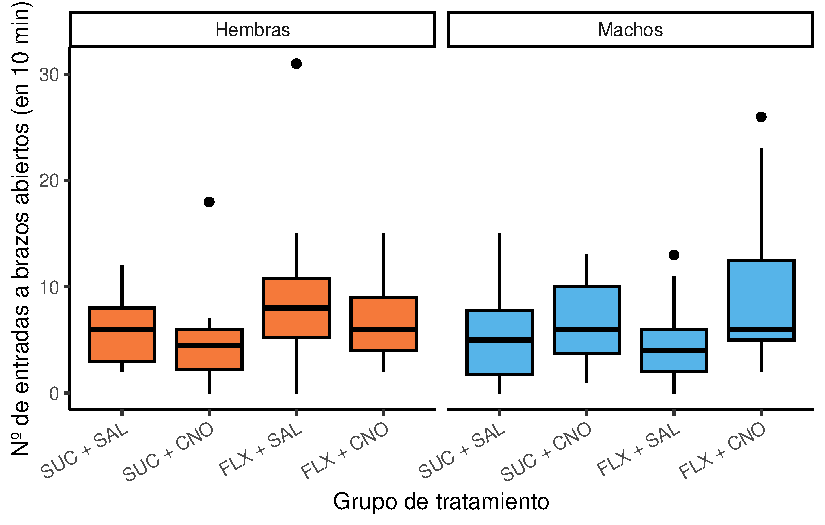
\includegraphics[keepaspectratio]{TP_Final_BIOME2_Informe_files/figure-pdf/boxplots-1.pdf}}

}

\caption{\textbf{Figura 1. Distribución del número de entradas a brazos
abiertos según el sexo y los tratamientos recibidos.} FLX: fluoxetina;
SUC: sacarosa (control); CNO:activador de los DREADDs; SAL: salina
(control). Cada caja resume la distribución de los datos del grupo
correspondiente.}

\end{figure}%

En el grafico de boxplots {[}Figura 1{]} se puede observar que, tanto en
hembras como en machos, las medianas de entradas a los brazos abiertos
se mantienen en un mismo rango (entre 4 y 8) entre los grupos de
tratamiento. También, se observa una mayor dispersión de los datos en
los machos que en las hembras (particularmente marcada hacia valores
altos en el grupo FLX + CNO), además de registrarse algunos valores
atípicos elevados en ambos sexos.

\begin{Shaded}
\begin{Highlighting}[]
\NormalTok{p5 }\OtherTok{\textless{}{-}} \FunctionTok{ggplot}\NormalTok{(Datos, }\FunctionTok{aes}\NormalTok{(}\AttributeTok{x =}\NormalTok{ FLX\_SUC,}
                        \AttributeTok{y =}\NormalTok{ Brazos\_abiertos\_entradas,}
                        \AttributeTok{colour =}\NormalTok{ SAL\_CNO,}
                        \AttributeTok{fill =}\NormalTok{ SAL\_CNO,}
                        \AttributeTok{group =}\NormalTok{ SAL\_CNO)) }\SpecialCharTok{+}
  \FunctionTok{geom\_jitter}\NormalTok{(}\AttributeTok{shape =} \DecValTok{21}\NormalTok{,}
              \AttributeTok{colour =} \StringTok{"white"}\NormalTok{,}
              \AttributeTok{stroke =} \FloatTok{0.3}\NormalTok{,}
              \AttributeTok{width =} \FloatTok{0.08}\NormalTok{,}
              \AttributeTok{height =} \DecValTok{0}\NormalTok{,}
              \AttributeTok{size =} \DecValTok{2}\NormalTok{,}
              \AttributeTok{alpha =} \FloatTok{0.8}\NormalTok{) }\SpecialCharTok{+}
  \FunctionTok{stat\_summary}\NormalTok{(}\AttributeTok{fun =}\NormalTok{ mean, }\AttributeTok{geom =} \StringTok{"line"}\NormalTok{, }\AttributeTok{linewidth =} \DecValTok{1}\NormalTok{) }\SpecialCharTok{+}
  \FunctionTok{stat\_summary}\NormalTok{(}\AttributeTok{fun =}\NormalTok{ mean, }\AttributeTok{geom =} \StringTok{"point"}\NormalTok{,}
               \AttributeTok{shape =} \DecValTok{21}\NormalTok{, }\AttributeTok{size =} \DecValTok{2}\NormalTok{, }\AttributeTok{stroke =} \FloatTok{1.5}\NormalTok{) }\SpecialCharTok{+}
  \FunctionTok{facet\_wrap}\NormalTok{(}\SpecialCharTok{\textasciitilde{}}\NormalTok{sexo,}
             \AttributeTok{labeller =} \FunctionTok{as\_labeller}\NormalTok{(}\FunctionTok{c}\NormalTok{(}\AttributeTok{macho =} \StringTok{"Machos"}\NormalTok{,}
                                      \AttributeTok{hembra =} \StringTok{"Hembras"}\NormalTok{))) }\SpecialCharTok{+}
  \FunctionTok{scale\_colour\_manual}\NormalTok{(}
    \AttributeTok{values =} \FunctionTok{c}\NormalTok{(}\StringTok{"SAL"} \OtherTok{=} \StringTok{"\#2B7BBF"}\NormalTok{,}
               \StringTok{"CNO"} \OtherTok{=} \StringTok{"\#C4501B"}\NormalTok{),}
    \AttributeTok{labels =} \FunctionTok{c}\NormalTok{(}\StringTok{"SAL"} \OtherTok{=} \StringTok{"Salina"}\NormalTok{,}
               \StringTok{"CNO"} \OtherTok{=} \StringTok{"CNO"}\NormalTok{)}
\NormalTok{  ) }\SpecialCharTok{+}
  \FunctionTok{scale\_fill\_manual}\NormalTok{(}
    \AttributeTok{values =} \FunctionTok{c}\NormalTok{(}\StringTok{"SAL"} \OtherTok{=} \StringTok{"\#85C0F9"}\NormalTok{,}
               \StringTok{"CNO"} \OtherTok{=} \StringTok{"\#F5793A"}\NormalTok{),}
    \AttributeTok{labels =} \FunctionTok{c}\NormalTok{(}\StringTok{"SAL"} \OtherTok{=} \StringTok{"Salina"}\NormalTok{,}
               \StringTok{"CNO"} \OtherTok{=} \StringTok{"CNO"}\NormalTok{)}
\NormalTok{  ) }\SpecialCharTok{+}
  \FunctionTok{xlab}\NormalTok{(}\StringTok{"Tratamiento"}\NormalTok{) }\SpecialCharTok{+}
  \FunctionTok{ylab}\NormalTok{(}\StringTok{"N° promedio de entradas a brazos abiertos"}\NormalTok{) }\SpecialCharTok{+}
  \FunctionTok{ggtitle}\NormalTok{(}\StringTok{"Entradas a brazos abiertos vs. tratamiento"}\NormalTok{) }\SpecialCharTok{+}
  \FunctionTok{labs}\NormalTok{(}\AttributeTok{colour =} \StringTok{"Administración de CNO"}\NormalTok{,}
       \AttributeTok{fill =} \StringTok{"Administración de CNO"}\NormalTok{)}

\NormalTok{p5}
\end{Highlighting}
\end{Shaded}

\begin{figure}[H]

{\centering \pandocbounded{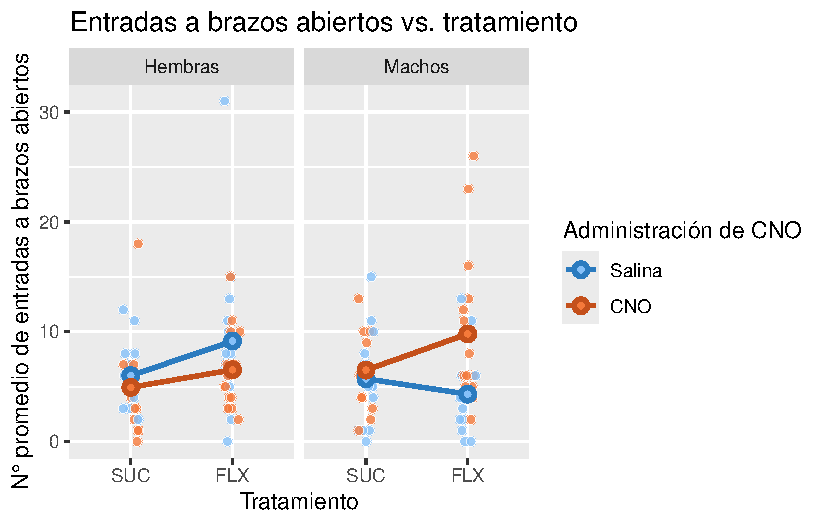
\includegraphics[keepaspectratio]{TP_Final_BIOME2_Informe_files/figure-pdf/gráfico de perfiles-1.pdf}}

}

\caption{\textbf{Figura 2. Gráfico de perfiles del número promedio de
entradas a brazos abiertos (en 10 minutos) según el sexo y los
tratamientos recibidos.} Los puntos grandes indican la media de cada
grupo y los puntos pequeños, los datos individuales. El color indica la
administración de CNO (azul: salina; naranja: CNO).}

\end{figure}%

En el gráfico de perfiles {[}Figura 2{]} se puede observar que, dentro
de los ratones tratados con SAL, el efecto de la Fluoxetina sobre las
entradas a brazos abiertos parecería variar entre sexos, dado que se
puede apreciar un aumento en la media de ingresos en hembras tratadas
con FLX respecto a SUC y una disminución en machos. Por otra parte, en
aquellos individuos tratados con CNO, se observa un aumento en la media
de ingresos en ambos sexos, aunque más pronunciada en el caso de los
machos.

\subsubsection{\texorpdfstring{\textbf{Modelo de
Poisson}}{Modelo de Poisson}}\label{modelo-de-poisson}

Debido a que la variable respuesta es un conteo en un continuo temporal,
se propuso inicialmente ajustar el modelo a una distribución de Poisson
con función de enlace log.

\paragraph{\texorpdfstring{\textbf{Especificación y supuestos
distribucionales}}{Especificación y supuestos distribucionales}}\label{especificaciuxf3n-y-supuestos-distribucionales}

\[\begin{aligned}
logE(Y_{ijkl}) = {} & \beta_0 + \beta_1 \text{FLX}_i + \beta_2 \text{CNO}_j + \beta_3\text{macho}_k + \beta_4 (\text{FLX} \times \text{CNO})_{ij} + \beta_5 (\text{FLX} \times \text{macho})_{ik}\\
& + \beta_6 (\text{CNO} \times \text{macho})_{jk} + \beta_7 (\text{FLX} \times \text{CNO} \times \text{macho})_{ijk} + C_{l(ij)}
\end{aligned}\]

\[Y_{ijkl} \approx \text{Poisson}(\lambda_{ijkl}), \quad \text{E}(Y_{ijkl}) = \text{Var}(Y_{ijkl}) = \lambda_{ijkl} = \mu_{ijkl}\]

\[C_{l(ij)} \sim NID(0,\sigma_\text{camada}^2)\]

La interacción triple contempla que el efecto de FLX difiere según la
administración de CNO y según el sexo, mientras que el efecto aleatorio
de camada contempla que los ratones de una misma camada no son
independientes entre sí.

\begin{Shaded}
\begin{Highlighting}[]
\NormalTok{modelo1 }\OtherTok{\textless{}{-}} \FunctionTok{glmmTMB}\NormalTok{(}
\NormalTok{  Brazos\_abiertos\_entradas }\SpecialCharTok{\textasciitilde{}}\NormalTok{ FLX\_SUC }\SpecialCharTok{*}\NormalTok{ SAL\_CNO }\SpecialCharTok{*}\NormalTok{ sexo }\SpecialCharTok{+}\NormalTok{ (}\DecValTok{1} \SpecialCharTok{|}\NormalTok{ camada),}
  \AttributeTok{data =}\NormalTok{ Datos,}
  \AttributeTok{family =} \FunctionTok{poisson}\NormalTok{(}\AttributeTok{link =} \StringTok{"log"}\NormalTok{))}

\FunctionTok{summary}\NormalTok{(modelo1)}
\end{Highlighting}
\end{Shaded}

\begin{verbatim}
 Family: poisson  ( log )
Formula:          
Brazos_abiertos_entradas ~ FLX_SUC * SAL_CNO * sexo + (1 | camada)
Data: Datos

      AIC       BIC    logLik -2*log(L)  df.resid 
    701.7     726.1    -341.9     683.7       101 

Random effects:

Conditional model:
 Groups Name        Variance Std.Dev.
 camada (Intercept) 0.1098   0.3314  
Number of obs: 110, groups:  camada, 20

Conditional model:
                                Estimate Std. Error z value Pr(>|z|)    
(Intercept)                      1.79798    0.21312   8.436   <2e-16 ***
FLX_SUCFLX                       0.38435    0.27248   1.411   0.1584    
SAL_CNOCNO                      -0.31699    0.29962  -1.058   0.2901    
sexomacho                       -0.19668    0.18991  -1.036   0.3004    
FLX_SUCFLX:SAL_CNOCNO           -0.03106    0.38289  -0.081   0.9354    
FLX_SUCFLX:sexomacho            -0.60126    0.25447  -2.363   0.0181 *  
SAL_CNOCNO:sexomacho             0.59803    0.26081   2.293   0.0219 *  
FLX_SUCFLX:SAL_CNOCNO:sexomacho  0.59405    0.33724   1.762   0.0782 .  
---
Signif. codes:  0 '***' 0.001 '**' 0.01 '*' 0.05 '.' 0.1 ' ' 1
\end{verbatim}

\paragraph{\texorpdfstring{\textbf{Diagnóstico:
SOBREDISPERSIÓN}}{Diagnóstico: SOBREDISPERSIÓN}}\label{diagnuxf3stico-sobredispersiuxf3n}

En el modelo de Poisson se asume \(\text{Var}(Y_{ijkl}) = \mu_{ijkl}\) y
un valor cercano a 1 del estadístico de dispersión es consistente con el
supuesto; valores \(≫1\) indican sobredispersión.

\begin{Shaded}
\begin{Highlighting}[]
\NormalTok{residuos\_m1 }\OtherTok{\textless{}{-}} \FunctionTok{simulateResiduals}\NormalTok{(modelo1)          }\CommentTok{\# Simulamos residuos con DHARMa}

\FunctionTok{plot}\NormalTok{(residuos\_m1)}
\end{Highlighting}
\end{Shaded}

\pandocbounded{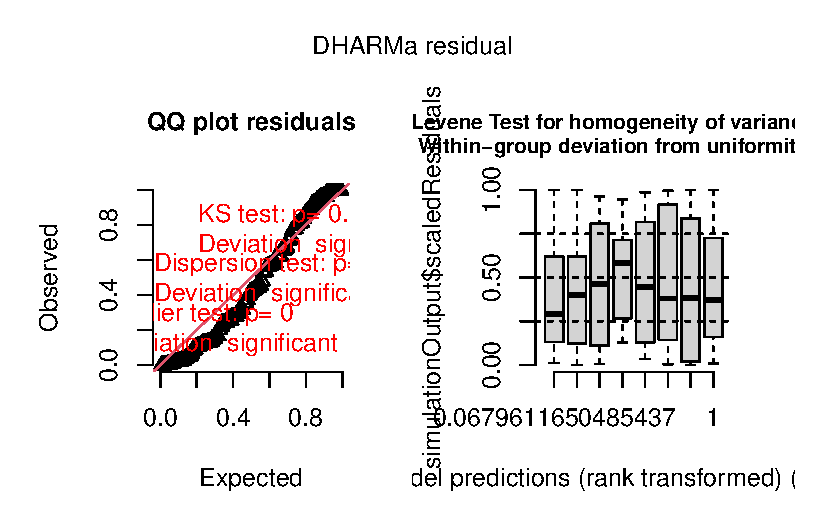
\includegraphics[keepaspectratio]{TP_Final_BIOME2_Informe_files/figure-pdf/unnamed-chunk-8-1.pdf}}

Diagnóstico DHARMa para el modelo de Poisson. El Q-Q plot (izquierda)
muestra desviaciones respecto a la distribución uniforme esperada bajo
el modelo. El gráfico de residuos contra predicciones (derecha) no
muestra evidencia de heterogeneidad de varianzas entre grupos (test de
Levene n.s.).

\begin{Shaded}
\begin{Highlighting}[]
\FunctionTok{testDispersion}\NormalTok{(residuos\_m1)                        }\CommentTok{\# Test dispersión}
\end{Highlighting}
\end{Shaded}

\pandocbounded{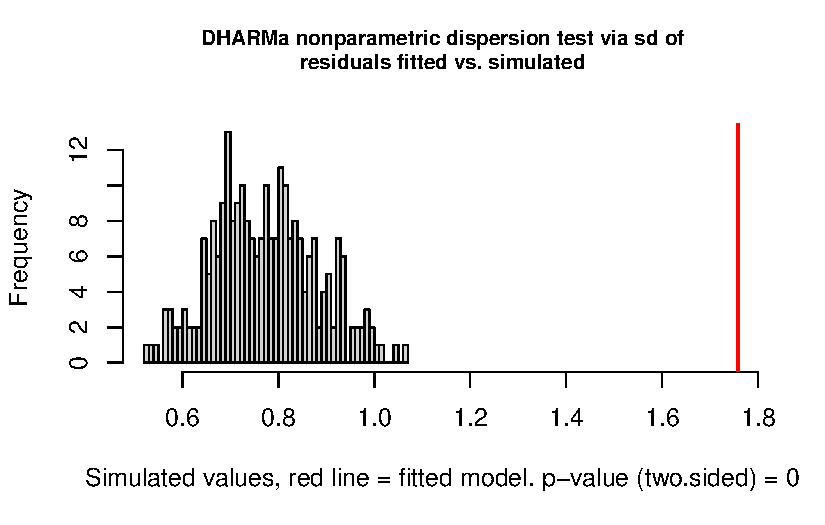
\includegraphics[keepaspectratio]{TP_Final_BIOME2_Informe_files/figure-pdf/unnamed-chunk-9-1.pdf}}

\begin{verbatim}

    DHARMa nonparametric dispersion test via sd of residuals fitted vs.
    simulated

data:  simulationOutput
dispersion = 2.2753, p-value < 2.2e-16
alternative hypothesis: two.sided
\end{verbatim}

La dispersión observada (línea roja) supera la esperada bajo el modelo
de Poisson (histograma), lo que indica sobredispersión (dispersión =
2.28, p \textless{} 2.2e-16).

Luego, el test de inflación de ceros de DHARMa indicó que el modelo de
Poisson subestima la cantidad de ceros observados (5 observados frente a
\textasciitilde1 esperado; razón observado/simulado = 5.66, p
\textless{} 2.2e16), lo que es coherente con la sobredispersión
detectada.

\begin{tcolorbox}[enhanced jigsaw, arc=.35mm, bottomrule=.15mm, breakable, colback=white, colframe=quarto-callout-note-color-frame, left=2mm, leftrule=.75mm, opacityback=0, rightrule=.15mm, toprule=.15mm]
\begin{minipage}[t]{5.5mm}
\textcolor{quarto-callout-note-color}{\faInfo}
\end{minipage}%
\begin{minipage}[t]{\textwidth - 5.5mm}

\vspace{-3mm}\textbf{Ver código}\vspace{3mm}

\begin{Shaded}
\begin{Highlighting}[]
\FunctionTok{testZeroInflation}\NormalTok{(residuos\_m1)                     }\CommentTok{\# Test inflación en ceros}
\end{Highlighting}
\end{Shaded}

\pandocbounded{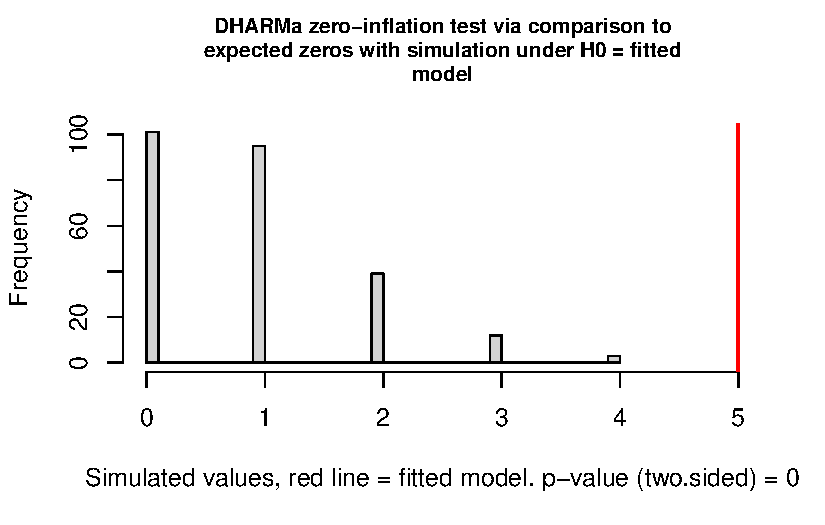
\includegraphics[keepaspectratio]{TP_Final_BIOME2_Informe_files/figure-pdf/ceros-m1-1.pdf}}

\begin{verbatim}

    DHARMa zero-inflation test via comparison to expected zeros with
    simulation under H0 = fitted model

data:  simulationOutput
ratioObsSim = 5.6561, p-value < 2.2e-16
alternative hypothesis: two.sided
\end{verbatim}

\end{minipage}%
\end{tcolorbox}

También, en los residuos de DHARMa frente a las predicciones del modelo
de Poisson se detectan desviaciones de los cuantiles (curva roja) con
observaciones atípicas en los extremos (asteriscos rojos), lo que es
coherente con la sobredispersión observada.

\begin{tcolorbox}[enhanced jigsaw, arc=.35mm, bottomrule=.15mm, breakable, colback=white, colframe=quarto-callout-note-color-frame, left=2mm, leftrule=.75mm, opacityback=0, rightrule=.15mm, toprule=.15mm]
\begin{minipage}[t]{5.5mm}
\textcolor{quarto-callout-note-color}{\faInfo}
\end{minipage}%
\begin{minipage}[t]{\textwidth - 5.5mm}

\vspace{-3mm}\textbf{Ver código}\vspace{3mm}

\begin{Shaded}
\begin{Highlighting}[]
\FunctionTok{plotResiduals}\NormalTok{(residuos\_m1, }\AttributeTok{form =} \FunctionTok{fitted}\NormalTok{(modelo1)) }\CommentTok{\# Residuos frente a valores ajustados}
\end{Highlighting}
\end{Shaded}

\pandocbounded{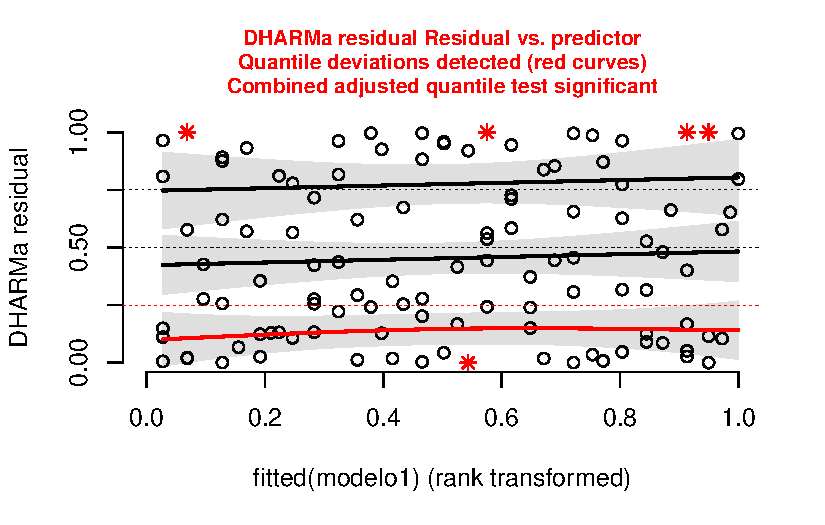
\includegraphics[keepaspectratio]{TP_Final_BIOME2_Informe_files/figure-pdf/residuos-ajustados-m1-1.pdf}}

\end{minipage}%
\end{tcolorbox}

Y por último, en el test de valores atípicos de DHARMa para el modelo de
Poisson se indica con las barras rojas que hay observaciones fuera del
rango de los datos simulados (5 de 110; frecuencia observada = 0.045
frente a 0.007 esperada, p \textless{} 2.2e-16), lo que es coherente con
la sobredispersión.

\begin{tcolorbox}[enhanced jigsaw, arc=.35mm, bottomrule=.15mm, breakable, colback=white, colframe=quarto-callout-note-color-frame, left=2mm, leftrule=.75mm, opacityback=0, rightrule=.15mm, toprule=.15mm]
\begin{minipage}[t]{5.5mm}
\textcolor{quarto-callout-note-color}{\faInfo}
\end{minipage}%
\begin{minipage}[t]{\textwidth - 5.5mm}

\vspace{-3mm}\textbf{Ver código}\vspace{3mm}

\begin{Shaded}
\begin{Highlighting}[]
\FunctionTok{testOutliers}\NormalTok{(residuos\_m1)                          }\CommentTok{\# Test Outliers}
\end{Highlighting}
\end{Shaded}

\pandocbounded{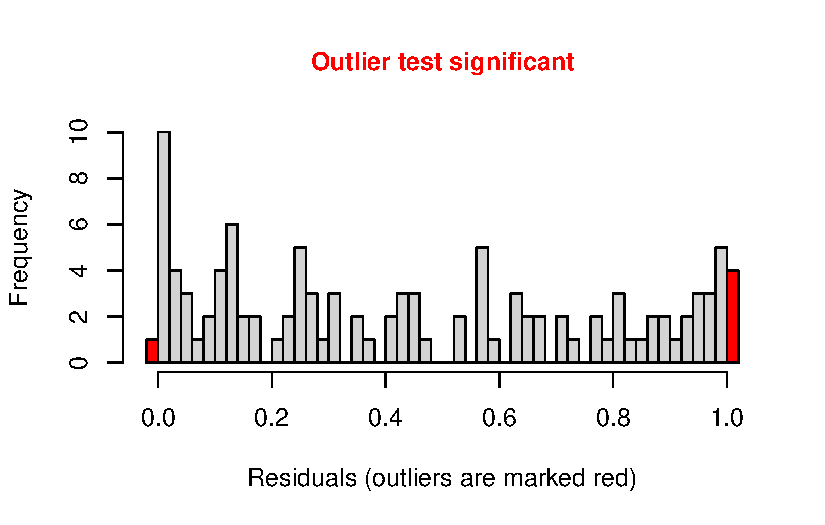
\includegraphics[keepaspectratio]{TP_Final_BIOME2_Informe_files/figure-pdf/outliers-m1-1.pdf}}

\begin{verbatim}

    DHARMa bootstrapped outlier test

data:  residuos_m1
outliers at both margin(s) = 5, observations = 110, p-value < 2.2e-16
alternative hypothesis: two.sided
 percent confidence interval:
 0.00000000 0.02727273
sample estimates:
outlier frequency (expected: 0.00754545454545455 ) 
                                        0.04545455 
\end{verbatim}

\end{minipage}%
\end{tcolorbox}

También, de forma manual se calcula el estadístico de dispersión

\begin{Shaded}
\begin{Highlighting}[]
\CommentTok{\# Calculamos estadístico de dispersión manualmente}
\FunctionTok{sum}\NormalTok{(}\FunctionTok{residuals}\NormalTok{(modelo1, }\AttributeTok{type=}\StringTok{"pearson"}\NormalTok{)}\SpecialCharTok{\^{}}\DecValTok{2}\NormalTok{)}\SpecialCharTok{/}\FunctionTok{df.residual}\NormalTok{(modelo1)}
\end{Highlighting}
\end{Shaded}

\begin{verbatim}
[1] 2.597938
\end{verbatim}

El estadístico de dispersión es superior al valor esperado de 1 bajo el
modelo de Poisson, lo que indica sobredispersión.

\begin{tcolorbox}[enhanced jigsaw, arc=.35mm, bottomrule=.15mm, bottomtitle=1mm, breakable, colback=white, colbacktitle=quarto-callout-important-color!10!white, colframe=quarto-callout-important-color-frame, coltitle=black, left=2mm, leftrule=.75mm, opacityback=0, opacitybacktitle=0.6, rightrule=.15mm, title=\textcolor{quarto-callout-important-color}{\faExclamation}\hspace{0.5em}{Sobredispersión confirmada}, titlerule=0mm, toprule=.15mm, toptitle=1mm]

Un estadístico de dispersión significativamente mayor a 1 y las
desviaciones en el Q-Q plot de DHARMa indican que la varianza observada
supera lo esperado bajo el modelo de Poisson. Por lo tanto, se decidió
continuar el análisis ajustando con otros modelos que incorporen un
parámetro adicional de dispersión.

\end{tcolorbox}

Además de la sobredispersión, se evalúa el supuesto de normalidad de los
residuos aleatorios de las camadas, que en el modelo se asumen
distribuidos normalmente con media 0 y varianza σ². Y se concluye que no
hay evidencia suficiente para rechazar que los residuos aleatorios de
las camadas siguen una distribución normal.

\begin{tcolorbox}[enhanced jigsaw, arc=.35mm, bottomrule=.15mm, breakable, colback=white, colframe=quarto-callout-note-color-frame, left=2mm, leftrule=.75mm, opacityback=0, rightrule=.15mm, toprule=.15mm]
\begin{minipage}[t]{5.5mm}
\textcolor{quarto-callout-note-color}{\faInfo}
\end{minipage}%
\begin{minipage}[t]{\textwidth - 5.5mm}

\vspace{-3mm}\textbf{Ver código}\vspace{3mm}

\begin{Shaded}
\begin{Highlighting}[]
\NormalTok{ef\_camadas\_m1 }\OtherTok{\textless{}{-}} \FunctionTok{ranef}\NormalTok{(modelo1)}\SpecialCharTok{$}\NormalTok{cond}\SpecialCharTok{$}\NormalTok{camada[[}\StringTok{"(Intercept)"}\NormalTok{]]}

\FunctionTok{qqPlot}\NormalTok{(}
\NormalTok{  ef\_camadas\_m1,}
  \AttributeTok{main =} \StringTok{"QQ Plot de efectos aleatorios de las camadas"}\NormalTok{,}
  \AttributeTok{ylab =} \StringTok{"Efectos aleatorios estimados"}
\NormalTok{)}
\end{Highlighting}
\end{Shaded}

\pandocbounded{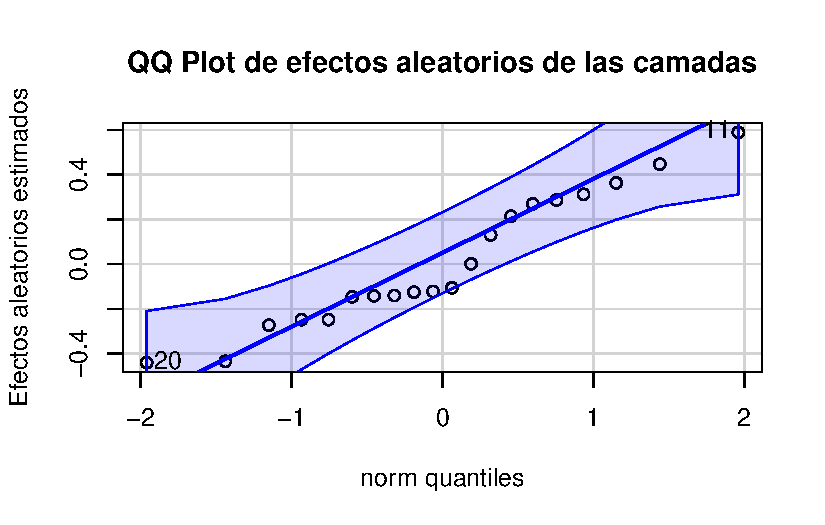
\includegraphics[keepaspectratio]{TP_Final_BIOME2_Informe_files/figure-pdf/efectos-aleatorios-m1-1.pdf}}

\begin{verbatim}
[1] 11 20
\end{verbatim}

\begin{Shaded}
\begin{Highlighting}[]
\FunctionTok{shapiro.test}\NormalTok{(ef\_camadas\_m1)       }\CommentTok{\# Shapiro{-}Wilk test}
\end{Highlighting}
\end{Shaded}

\begin{verbatim}

    Shapiro-Wilk normality test

data:  ef_camadas_m1
W = 0.94325, p-value = 0.276
\end{verbatim}

\end{minipage}%
\end{tcolorbox}

\subsubsection{\texorpdfstring{\textbf{Modelos alternativos para
sobredispersión}}{Modelos alternativos para sobredispersión}}\label{modelos-alternativos-para-sobredispersiuxf3n}

\paragraph{\texorpdfstring{\textbf{Binomial negativa
(NB2)}}{Binomial negativa (NB2)}}\label{binomial-negativa-nb2}

\begin{Shaded}
\begin{Highlighting}[]
\NormalTok{modelo2 }\OtherTok{\textless{}{-}} \FunctionTok{glmmTMB}\NormalTok{(}
\NormalTok{  Brazos\_abiertos\_entradas }\SpecialCharTok{\textasciitilde{}}\NormalTok{ FLX\_SUC }\SpecialCharTok{*}\NormalTok{ SAL\_CNO }\SpecialCharTok{*}\NormalTok{ sexo }\SpecialCharTok{+}\NormalTok{ (}\DecValTok{1} \SpecialCharTok{|}\NormalTok{ camada),}
  \AttributeTok{family =} \StringTok{"nbinom2"}\NormalTok{,}
  \AttributeTok{data =}\NormalTok{ Datos}
\NormalTok{)}
\end{Highlighting}
\end{Shaded}

\subparagraph{\texorpdfstring{\textbf{Supuestos}}{Supuestos}}\label{supuestos}

El diagnóstico de residuos de DHARMa para el modelo de binomial negativa
no mostró evidencia de desviaciones respecto de la distribución uniforme
esperada (izquierda), ni de heterogeneidad de varianzas entre grupos
(derecha). Tampoco hay evidencia para rechazar que los residuos
aleatorios de las camadas siguen una distribución normal.

\begin{tcolorbox}[enhanced jigsaw, arc=.35mm, bottomrule=.15mm, breakable, colback=white, colframe=quarto-callout-note-color-frame, left=2mm, leftrule=.75mm, opacityback=0, rightrule=.15mm, toprule=.15mm]
\begin{minipage}[t]{5.5mm}
\textcolor{quarto-callout-note-color}{\faInfo}
\end{minipage}%
\begin{minipage}[t]{\textwidth - 5.5mm}

\vspace{-3mm}\textbf{Ver código}\vspace{3mm}

\begin{Shaded}
\begin{Highlighting}[]
\NormalTok{residuos\_m2 }\OtherTok{\textless{}{-}} \FunctionTok{simulateResiduals}\NormalTok{(modelo2)          }\CommentTok{\# Simulamos residuos con DHARMa}
\FunctionTok{plot}\NormalTok{(residuos\_m2)}
\end{Highlighting}
\end{Shaded}

\pandocbounded{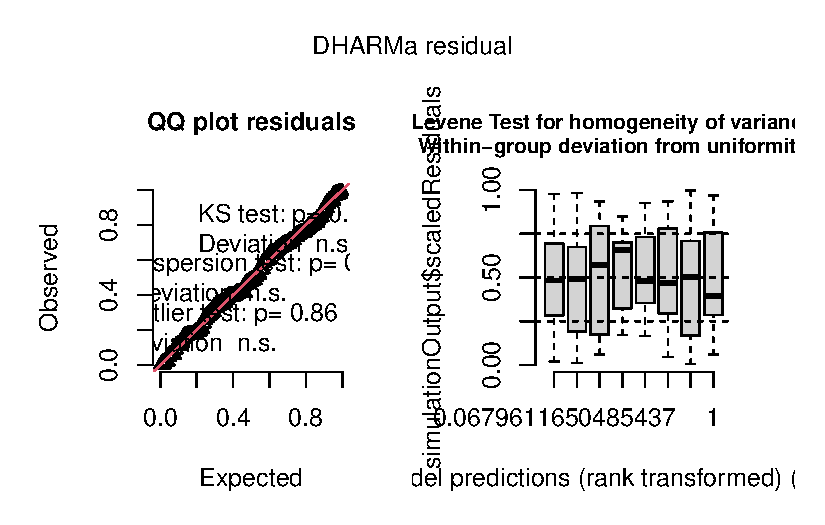
\includegraphics[keepaspectratio]{TP_Final_BIOME2_Informe_files/figure-pdf/diagnostico-m2-1.pdf}}

\end{minipage}%
\end{tcolorbox}

\begin{tcolorbox}[enhanced jigsaw, arc=.35mm, bottomrule=.15mm, breakable, colback=white, colframe=quarto-callout-note-color-frame, left=2mm, leftrule=.75mm, opacityback=0, rightrule=.15mm, toprule=.15mm]
\begin{minipage}[t]{5.5mm}
\textcolor{quarto-callout-note-color}{\faInfo}
\end{minipage}%
\begin{minipage}[t]{\textwidth - 5.5mm}

\vspace{-3mm}\textbf{Ver código}\vspace{3mm}

\begin{Shaded}
\begin{Highlighting}[]
\NormalTok{ef\_camadas\_m2 }\OtherTok{\textless{}{-}} \FunctionTok{ranef}\NormalTok{(modelo2)}\SpecialCharTok{$}\NormalTok{cond}\SpecialCharTok{$}\NormalTok{camada[[}\StringTok{"(Intercept)"}\NormalTok{]]}

\FunctionTok{qqPlot}\NormalTok{(}
\NormalTok{  ef\_camadas\_m2,}
  \AttributeTok{main =} \StringTok{"QQ Plot de efectos aleatorios de las camadas"}\NormalTok{,}
  \AttributeTok{ylab =} \StringTok{"Efectos aleatorios estimados"}
\NormalTok{)}
\end{Highlighting}
\end{Shaded}

\pandocbounded{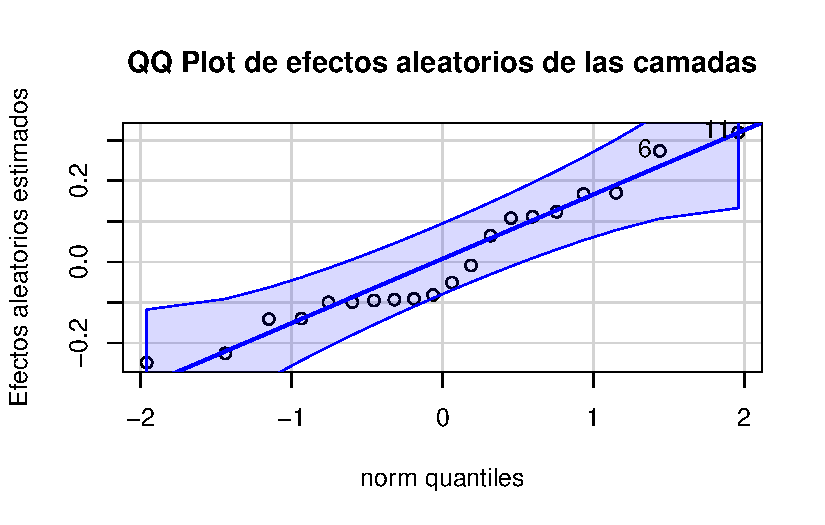
\includegraphics[keepaspectratio]{TP_Final_BIOME2_Informe_files/figure-pdf/efectos-aleatorios-m2-1.pdf}}

\begin{verbatim}
[1] 11  6
\end{verbatim}

\begin{Shaded}
\begin{Highlighting}[]
\FunctionTok{shapiro.test}\NormalTok{(ef\_camadas\_m2)       }\CommentTok{\# Shapiro{-}Wilk test}
\end{Highlighting}
\end{Shaded}

\begin{verbatim}

    Shapiro-Wilk normality test

data:  ef_camadas_m2
W = 0.93929, p-value = 0.2325
\end{verbatim}

\end{minipage}%
\end{tcolorbox}

\paragraph{\texorpdfstring{\textbf{Conway-Maxwell-Poisson
(CMP)}}{Conway-Maxwell-Poisson (CMP)}}\label{conway-maxwell-poisson-cmp}

\begin{Shaded}
\begin{Highlighting}[]
\NormalTok{modelo3 }\OtherTok{\textless{}{-}} \FunctionTok{glmmTMB}\NormalTok{(}
\NormalTok{  Brazos\_abiertos\_entradas }\SpecialCharTok{\textasciitilde{}}\NormalTok{ FLX\_SUC }\SpecialCharTok{*}\NormalTok{ SAL\_CNO }\SpecialCharTok{*}\NormalTok{ sexo }\SpecialCharTok{+}\NormalTok{ (}\DecValTok{1} \SpecialCharTok{|}\NormalTok{ camada),}
  \AttributeTok{family =} \StringTok{"compois"}\NormalTok{,}
  \AttributeTok{data =}\NormalTok{ Datos}
\NormalTok{)}
\end{Highlighting}
\end{Shaded}

\subparagraph{\texorpdfstring{\textbf{Supuestos}}{Supuestos}}\label{supuestos-1}

El diagnóstico de residuos de DHARMa para el modelo de
Conway-Maxwell-Poisson no mostró evidencia de desviaciones respecto de
la distribución uniforme esperada (izquierda), ni de heterogeneidad de
varianzas entre grupos (derecha). Tampoco hay evidencia para rechazar
que los residuos aleatorios de las camadas siguen una distribución
normal.

\begin{tcolorbox}[enhanced jigsaw, arc=.35mm, bottomrule=.15mm, breakable, colback=white, colframe=quarto-callout-note-color-frame, left=2mm, leftrule=.75mm, opacityback=0, rightrule=.15mm, toprule=.15mm]
\begin{minipage}[t]{5.5mm}
\textcolor{quarto-callout-note-color}{\faInfo}
\end{minipage}%
\begin{minipage}[t]{\textwidth - 5.5mm}

\vspace{-3mm}\textbf{Ver código}\vspace{3mm}

\begin{Shaded}
\begin{Highlighting}[]
\NormalTok{residuos\_m3 }\OtherTok{\textless{}{-}} \FunctionTok{simulateResiduals}\NormalTok{(modelo3)          }\CommentTok{\# Simulamos residuos con DHARMa}
\FunctionTok{plot}\NormalTok{(residuos\_m3)}
\end{Highlighting}
\end{Shaded}

\pandocbounded{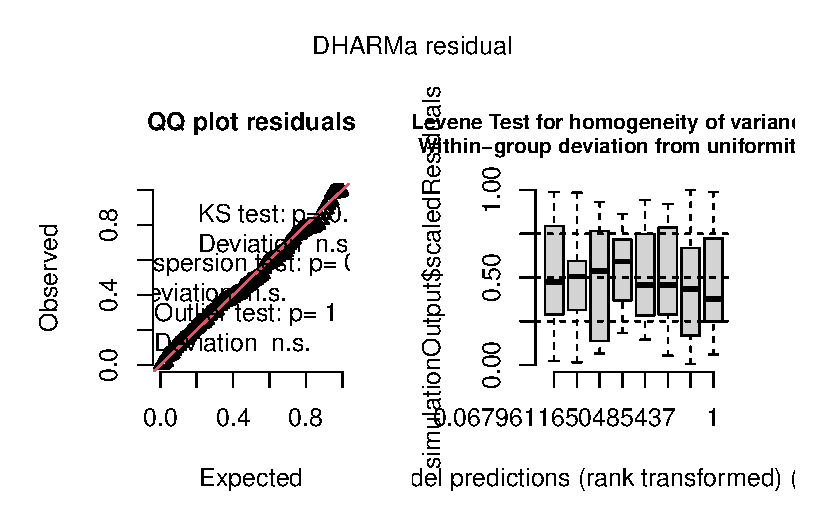
\includegraphics[keepaspectratio]{TP_Final_BIOME2_Informe_files/figure-pdf/diagnostico-m3-1.pdf}}

\end{minipage}%
\end{tcolorbox}

\begin{tcolorbox}[enhanced jigsaw, arc=.35mm, bottomrule=.15mm, breakable, colback=white, colframe=quarto-callout-note-color-frame, left=2mm, leftrule=.75mm, opacityback=0, rightrule=.15mm, toprule=.15mm]
\begin{minipage}[t]{5.5mm}
\textcolor{quarto-callout-note-color}{\faInfo}
\end{minipage}%
\begin{minipage}[t]{\textwidth - 5.5mm}

\vspace{-3mm}\textbf{Ver código}\vspace{3mm}

\begin{Shaded}
\begin{Highlighting}[]
\NormalTok{ef\_camadas\_m3 }\OtherTok{\textless{}{-}} \FunctionTok{ranef}\NormalTok{(modelo3)}\SpecialCharTok{$}\NormalTok{cond}\SpecialCharTok{$}\NormalTok{camada[[}\StringTok{"(Intercept)"}\NormalTok{]]}

\FunctionTok{qqPlot}\NormalTok{(}
\NormalTok{  ef\_camadas\_m3,}
  \AttributeTok{main =} \StringTok{"QQ Plot de efectos aleatorios de las camadas"}\NormalTok{,}
  \AttributeTok{ylab =} \StringTok{"Efectos aleatorios estimados"}
\NormalTok{)}
\end{Highlighting}
\end{Shaded}

\pandocbounded{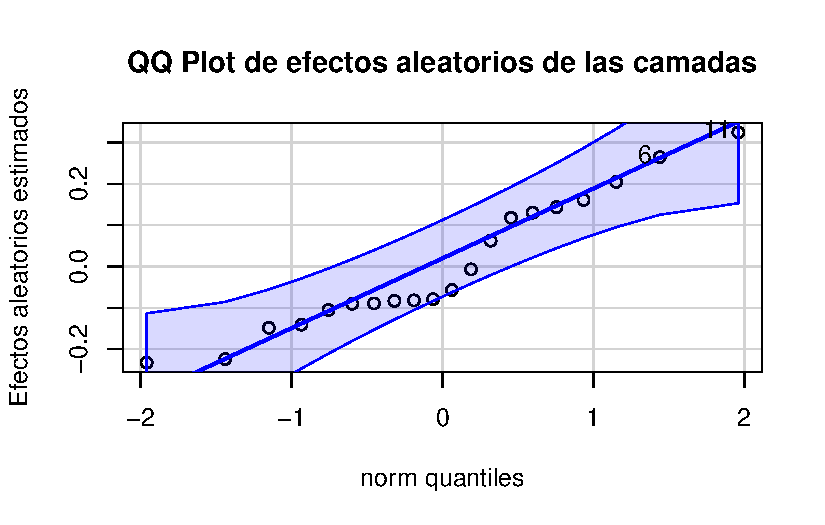
\includegraphics[keepaspectratio]{TP_Final_BIOME2_Informe_files/figure-pdf/efectos-aleatorios-m3-1.pdf}}

\begin{verbatim}
[1] 11  6
\end{verbatim}

\begin{Shaded}
\begin{Highlighting}[]
\FunctionTok{shapiro.test}\NormalTok{(ef\_camadas\_m3)       }\CommentTok{\# Shapiro{-}Wilk test}
\end{Highlighting}
\end{Shaded}

\begin{verbatim}

    Shapiro-Wilk normality test

data:  ef_camadas_m3
W = 0.9358, p-value = 0.1995
\end{verbatim}

\end{minipage}%
\end{tcolorbox}

\paragraph{\texorpdfstring{\textbf{Tweedie}}{Tweedie}}\label{tweedie}

\begin{Shaded}
\begin{Highlighting}[]
\NormalTok{modelo4 }\OtherTok{\textless{}{-}} \FunctionTok{glmmTMB}\NormalTok{(}
\NormalTok{  Brazos\_abiertos\_entradas }\SpecialCharTok{\textasciitilde{}}\NormalTok{ FLX\_SUC }\SpecialCharTok{*}\NormalTok{ SAL\_CNO }\SpecialCharTok{*}\NormalTok{ sexo }\SpecialCharTok{+}\NormalTok{ (}\DecValTok{1} \SpecialCharTok{|}\NormalTok{ camada),}
  \AttributeTok{family =} \StringTok{"tweedie"}\NormalTok{,}
  \AttributeTok{data =}\NormalTok{ Datos}
\NormalTok{)}
\end{Highlighting}
\end{Shaded}

\subparagraph{\texorpdfstring{\textbf{Supuestos}}{Supuestos}}\label{supuestos-2}

El diagnóstico de residuos de DHARMa para el modelo de Tweedie no mostró
evidencia de desviaciones respecto de la distribución uniforme esperada
(izquierda), ni de heterogeneidad de varianzas entre grupos (derecha).
Tampoco hay evidencia para rechazar que los residuos aleatorios de las
camadas siguen una distribución normal.

\begin{tcolorbox}[enhanced jigsaw, arc=.35mm, bottomrule=.15mm, breakable, colback=white, colframe=quarto-callout-note-color-frame, left=2mm, leftrule=.75mm, opacityback=0, rightrule=.15mm, toprule=.15mm]
\begin{minipage}[t]{5.5mm}
\textcolor{quarto-callout-note-color}{\faInfo}
\end{minipage}%
\begin{minipage}[t]{\textwidth - 5.5mm}

\vspace{-3mm}\textbf{Ver código}\vspace{3mm}

\begin{Shaded}
\begin{Highlighting}[]
\NormalTok{residuos\_m4 }\OtherTok{\textless{}{-}} \FunctionTok{simulateResiduals}\NormalTok{(modelo4)          }\CommentTok{\# Simulamos residuos con DHARMa}
\FunctionTok{plot}\NormalTok{(residuos\_m4)}
\end{Highlighting}
\end{Shaded}

\pandocbounded{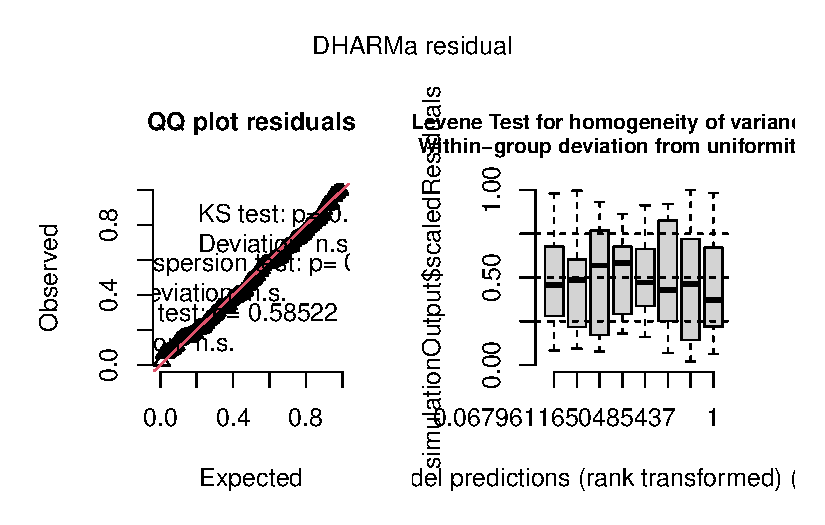
\includegraphics[keepaspectratio]{TP_Final_BIOME2_Informe_files/figure-pdf/diagnostico-m4-1.pdf}}

\end{minipage}%
\end{tcolorbox}

\begin{tcolorbox}[enhanced jigsaw, arc=.35mm, bottomrule=.15mm, breakable, colback=white, colframe=quarto-callout-note-color-frame, left=2mm, leftrule=.75mm, opacityback=0, rightrule=.15mm, toprule=.15mm]
\begin{minipage}[t]{5.5mm}
\textcolor{quarto-callout-note-color}{\faInfo}
\end{minipage}%
\begin{minipage}[t]{\textwidth - 5.5mm}

\vspace{-3mm}\textbf{Ver código}\vspace{3mm}

\begin{Shaded}
\begin{Highlighting}[]
\NormalTok{ef\_camadas\_m4 }\OtherTok{\textless{}{-}} \FunctionTok{ranef}\NormalTok{(modelo4)}\SpecialCharTok{$}\NormalTok{cond}\SpecialCharTok{$}\NormalTok{camada[[}\StringTok{"(Intercept)"}\NormalTok{]]}

\FunctionTok{qqPlot}\NormalTok{(}
\NormalTok{  ef\_camadas\_m4,}
  \AttributeTok{main =} \StringTok{"QQ Plot de efectos aleatorios de las camadas"}\NormalTok{,}
  \AttributeTok{ylab =} \StringTok{"Efectos aleatorios estimados"}
\NormalTok{)}
\end{Highlighting}
\end{Shaded}

\pandocbounded{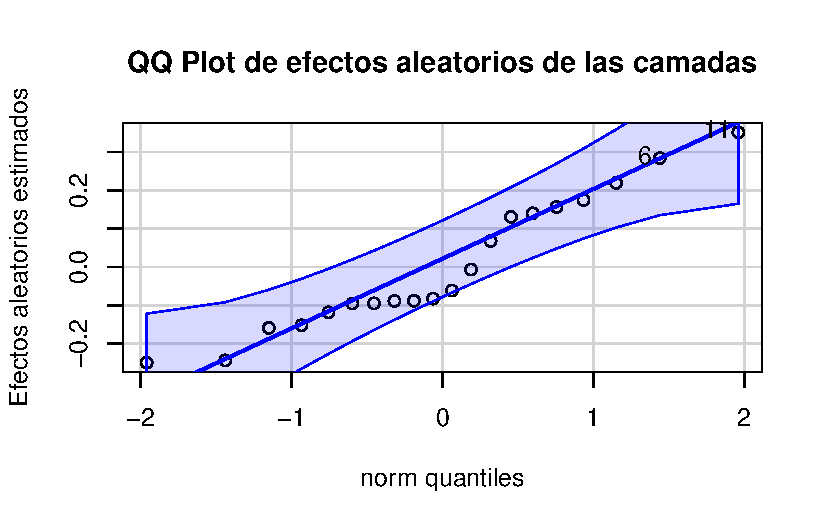
\includegraphics[keepaspectratio]{TP_Final_BIOME2_Informe_files/figure-pdf/efectos-aleatorios-m4-1.pdf}}

\begin{verbatim}
[1] 11  6
\end{verbatim}

\begin{Shaded}
\begin{Highlighting}[]
\FunctionTok{shapiro.test}\NormalTok{(ef\_camadas\_m4)       }\CommentTok{\# Shapiro{-}Wilk test}
\end{Highlighting}
\end{Shaded}

\begin{verbatim}

    Shapiro-Wilk normality test

data:  ef_camadas_m4
W = 0.93602, p-value = 0.2015
\end{verbatim}

\end{minipage}%
\end{tcolorbox}

\paragraph{\texorpdfstring{\textbf{OLRE}}{OLRE}}\label{olre}

\begin{Shaded}
\begin{Highlighting}[]
\NormalTok{modelo5 }\OtherTok{\textless{}{-}} \FunctionTok{glmmTMB}\NormalTok{(}
\NormalTok{  Brazos\_abiertos\_entradas }\SpecialCharTok{\textasciitilde{}}\NormalTok{ FLX\_SUC }\SpecialCharTok{*}\NormalTok{ SAL\_CNO }\SpecialCharTok{*}\NormalTok{ sexo }\SpecialCharTok{+}\NormalTok{ (}\DecValTok{1} \SpecialCharTok{|}\NormalTok{ camada) }\SpecialCharTok{+}\NormalTok{ (}\DecValTok{1} \SpecialCharTok{|}\NormalTok{ ID),}
  \AttributeTok{family =} \StringTok{"poisson"}\NormalTok{,}
  \AttributeTok{data =}\NormalTok{ Datos}
\NormalTok{)}
\end{Highlighting}
\end{Shaded}

\subparagraph{\texorpdfstring{\textbf{Supuestos}}{Supuestos}}\label{supuestos-3}

El diagnóstico de residuos de DHARMa para el modelo de OLRE no mostró
evidencia de desviaciones respecto de la distribución uniforme esperada
(izquierda), ni de heterogeneidad de varianzas entre grupos (derecha).
Tampoco hay evidencia para rechazar que los residuos aleatorios de las
camadas siguen una distribución normal.

\begin{tcolorbox}[enhanced jigsaw, arc=.35mm, bottomrule=.15mm, breakable, colback=white, colframe=quarto-callout-note-color-frame, left=2mm, leftrule=.75mm, opacityback=0, rightrule=.15mm, toprule=.15mm]
\begin{minipage}[t]{5.5mm}
\textcolor{quarto-callout-note-color}{\faInfo}
\end{minipage}%
\begin{minipage}[t]{\textwidth - 5.5mm}

\vspace{-3mm}\textbf{Ver código}\vspace{3mm}

\begin{Shaded}
\begin{Highlighting}[]
\NormalTok{residuos\_m5 }\OtherTok{\textless{}{-}} \FunctionTok{simulateResiduals}\NormalTok{(modelo5, }\AttributeTok{simulateREs =} \StringTok{"unconditional"}\NormalTok{) }\CommentTok{\# Simulamos residuos con DHARMa}
\FunctionTok{plot}\NormalTok{(residuos\_m5)}
\end{Highlighting}
\end{Shaded}

\pandocbounded{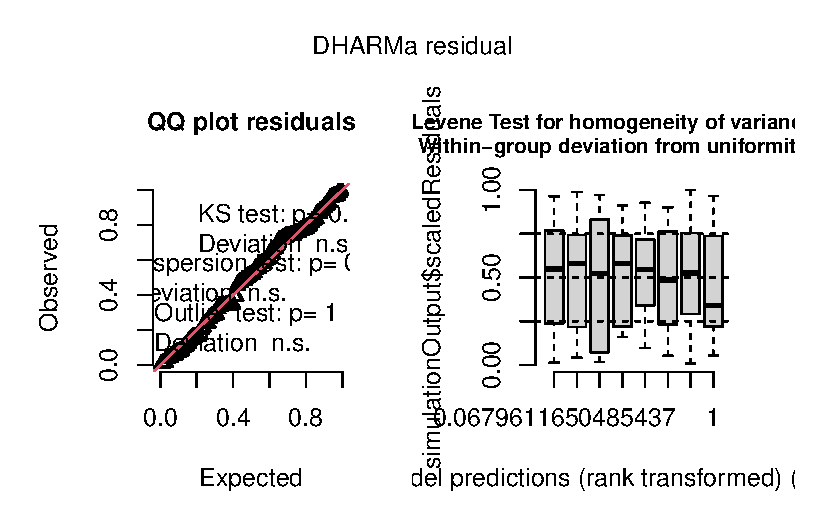
\includegraphics[keepaspectratio]{TP_Final_BIOME2_Informe_files/figure-pdf/diagnostico-m5-1.pdf}}

\end{minipage}%
\end{tcolorbox}

\begin{tcolorbox}[enhanced jigsaw, arc=.35mm, bottomrule=.15mm, breakable, colback=white, colframe=quarto-callout-note-color-frame, left=2mm, leftrule=.75mm, opacityback=0, rightrule=.15mm, toprule=.15mm]
\begin{minipage}[t]{5.5mm}
\textcolor{quarto-callout-note-color}{\faInfo}
\end{minipage}%
\begin{minipage}[t]{\textwidth - 5.5mm}

\vspace{-3mm}\textbf{Ver código}\vspace{3mm}

\begin{Shaded}
\begin{Highlighting}[]
\NormalTok{ef\_camadas\_m5 }\OtherTok{\textless{}{-}} \FunctionTok{ranef}\NormalTok{(modelo5)}\SpecialCharTok{$}\NormalTok{cond}\SpecialCharTok{$}\NormalTok{camada[[}\StringTok{"(Intercept)"}\NormalTok{]]}

\FunctionTok{qqPlot}\NormalTok{(}
\NormalTok{  ef\_camadas\_m5,}
  \AttributeTok{main =} \StringTok{"QQ Plot de efectos aleatorios de las camadas"}\NormalTok{,}
  \AttributeTok{ylab =} \StringTok{"Efectos aleatorios estimados"}
\NormalTok{)}
\end{Highlighting}
\end{Shaded}

\pandocbounded{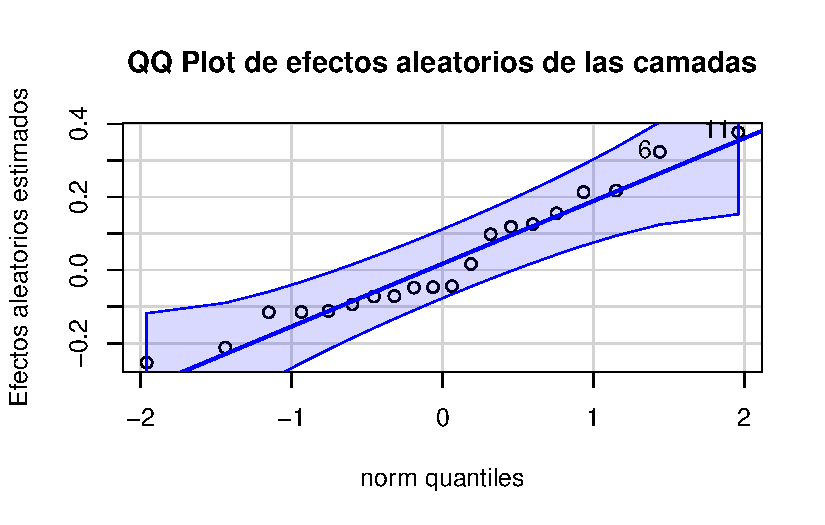
\includegraphics[keepaspectratio]{TP_Final_BIOME2_Informe_files/figure-pdf/efectos-aleatorios-m5-1.pdf}}

\begin{verbatim}
[1] 11  6
\end{verbatim}

\begin{Shaded}
\begin{Highlighting}[]
\FunctionTok{shapiro.test}\NormalTok{(ef\_camadas\_m5)       }\CommentTok{\# Shapiro{-}Wilk test}
\end{Highlighting}
\end{Shaded}

\begin{verbatim}

    Shapiro-Wilk normality test

data:  ef_camadas_m5
W = 0.94792, p-value = 0.3366
\end{verbatim}

\end{minipage}%
\end{tcolorbox}

\subsubsection{\texorpdfstring{\textbf{Comparación por
AIC}}{Comparación por AIC}}\label{comparaciuxf3n-por-aic}

Se selecciona el modelo con menor AIC entre aquellos con diagnóstico
DHARMa aceptable.

\begin{Shaded}
\begin{Highlighting}[]
\FunctionTok{AIC}\NormalTok{(modelo2, modelo3, modelo4, modelo5)}
\end{Highlighting}
\end{Shaded}

\begin{verbatim}
        df      AIC
modelo2 10 632.9165
modelo3 10 635.0152
modelo4 11 637.1339
modelo5 10 632.8728
\end{verbatim}

\begin{tcolorbox}[enhanced jigsaw, arc=.35mm, bottomrule=.15mm, bottomtitle=1mm, breakable, colback=white, colbacktitle=quarto-callout-tip-color!10!white, colframe=quarto-callout-tip-color-frame, coltitle=black, left=2mm, leftrule=.75mm, opacityback=0, opacitybacktitle=0.6, rightrule=.15mm, title=\textcolor{quarto-callout-tip-color}{\faLightbulb}\hspace{0.5em}{Selección del modelo}, titlerule=0mm, toprule=.15mm, toptitle=1mm]

Entre los modelos con menor AIC, OLRE y binomial negativa, se selecciona
\textbf{la binomial negativa} para el análisis de resultados.

\end{tcolorbox}

Para la evaluación global de los efectos fijos del modelo Binomial
Negativo seleccionado, se especifica una prueba de ANOVA de Devianza de
Wald Tipo III (car::Anova(\ldots, type = ``III'')). Debido al desbalance
muestral en las celdas experimentales y para garantizar el principio de
marginalidad e independencia respecto a la categoría de referencia
(baseline), el modelo se ajusta utilizando contrastes de suma cero
(contr.sum). A diferencia de la codificación de referencia por defecto
(donde el intercepto corresponde a una única combinación control y los
coeficientes expresan efectos simples condicionados a dicho nivel
basal), los contrastes de suma cero (contr.sum) reparametrizan el modelo
de manera simétrica (±1). Esto permite que el intercepto estime la media
general no ponderada del experimento y que cada efecto principal
cuantifique el desvío promedio de cada factor a través de todos los
niveles de los restantes factores, lo cual es indispensable para evaluar
adecuadamente la significancia global de los factores mediante sumas de
cuadrados tipo III en presencia de interacciones. Bajo esta
codificación, las variables dummy~ tienen un valor +1 en el primer nivel
de cada factor (FLX, SAL y Hembra, respectivamente) y -1 en el segundo
nivel (SUC, CNO y Macho).~

Utilizando este tipo de contrastes, cambia la interpretación de los
parámetros del modelo:

𝛽0 es el intercepto global en la escala logarítmica, correspondiente a
la media general no ponderada de todas las combinaciones experimentales.

𝛽1 representa el efecto principal del tratamiento con Fluoxetina
(desviación respecto a la media general, promediando entre tratamientos
CNO y sexo)

𝛽2 representa el efecto principal del tratamiento con CNO (desviación
respecto a la media general, promediando entre tratamientos Fluoxetina y
sexo).

𝛽3 representa el efecto principal del sexo (desviación respecto a la
media general, promediando entre tratamientos Fluoxetina y CNO).

𝛽4, 𝛽5, 𝛽6, 𝛽7 son los parámetros de interacción de doble y triple vía
en la escala del predictor lineal, que cuantifican las desviaciones no
aditivas respecto a los efectos principales.

\subsection{Resultados}\label{resultados}

\subsubsection{Modelo}\label{modelo}

\begin{tcolorbox}[enhanced jigsaw, arc=.35mm, bottomrule=.15mm, breakable, colback=white, colframe=quarto-callout-note-color-frame, left=2mm, leftrule=.75mm, opacityback=0, rightrule=.15mm, toprule=.15mm]
\begin{minipage}[t]{5.5mm}
\textcolor{quarto-callout-note-color}{\faInfo}
\end{minipage}%
\begin{minipage}[t]{\textwidth - 5.5mm}

\vspace{-3mm}\textbf{Ver código y summary}\vspace{3mm}

\begin{Shaded}
\begin{Highlighting}[]
\FunctionTok{options}\NormalTok{(}\AttributeTok{contrasts =} \FunctionTok{c}\NormalTok{(}\StringTok{"contr.sum"}\NormalTok{, }\StringTok{"contr.poly"}\NormalTok{))}
\NormalTok{modelo2 }\OtherTok{\textless{}{-}} \FunctionTok{glmmTMB}\NormalTok{(}
\NormalTok{  Brazos\_abiertos\_entradas }\SpecialCharTok{\textasciitilde{}}\NormalTok{ FLX\_SUC }\SpecialCharTok{*}\NormalTok{ SAL\_CNO }\SpecialCharTok{*}\NormalTok{ sexo }\SpecialCharTok{+}\NormalTok{ (}\DecValTok{1} \SpecialCharTok{|}\NormalTok{ camada),}
  \AttributeTok{family =} \StringTok{"nbinom2"}\NormalTok{,}
  \AttributeTok{data =}\NormalTok{ Datos}
\NormalTok{)}


\NormalTok{tabla.summary }\OtherTok{\textless{}{-}} \FunctionTok{summary}\NormalTok{(modelo2)}
\NormalTok{tabla.anova }\OtherTok{\textless{}{-}} \FunctionTok{Anova}\NormalTok{(modelo2, }\AttributeTok{type=}\StringTok{"III"}\NormalTok{)}

\FunctionTok{options}\NormalTok{(}\AttributeTok{contrasts =} \FunctionTok{c}\NormalTok{(}\StringTok{"contr.treatment"}\NormalTok{, }\StringTok{"contr.poly"}\NormalTok{))}

\NormalTok{tabla.summary}
\end{Highlighting}
\end{Shaded}

\begin{verbatim}
 Family: nbinom2  ( log )
Formula:          
Brazos_abiertos_entradas ~ FLX_SUC * SAL_CNO * sexo + (1 | camada)
Data: Datos

      AIC       BIC    logLik -2*log(L)  df.resid 
    632.9     659.9    -306.5     612.9       100 

Random effects:

Conditional model:
 Groups Name        Variance Std.Dev.
 camada (Intercept) 0.05914  0.2432  
Number of obs: 110, groups:  camada, 20

Dispersion parameter for nbinom2 family (): 3.61 

Conditional model:
                        Estimate Std. Error z value Pr(>|z|)    
(Intercept)              1.82576    0.08690  21.011  < 2e-16 ***
FLX_SUC1                -0.11358    0.08602  -1.320  0.18671    
SAL_CNO1                -0.05321    0.08597  -0.619  0.53592    
sexo1                    0.01694    0.06771   0.250  0.80248    
FLX_SUC1:SAL_CNO1        0.06279    0.08598   0.730  0.46522    
FLX_SUC1:sexo1          -0.08627    0.06817  -1.265  0.20570    
SAL_CNO1:sexo1           0.20787    0.06846   3.036  0.00239 ** 
FLX_SUC1:SAL_CNO1:sexo1 -0.07815    0.06853  -1.140  0.25412    
---
Signif. codes:  0 '***' 0.001 '**' 0.01 '*' 0.05 '.' 0.1 ' ' 1
\end{verbatim}

\end{minipage}%
\end{tcolorbox}

\[\begin{aligned}
logE(Y_{ijkl}) = {} & 1.82 -0.11 \text{ FLX}_i -0.05 \text{ CNO}_j + 0.01\text{ macho}_k + 0.06 (\text{FLX} \times \text{CNO})_{ij} \\
& -0.08 (\text{FLX} \times \text{macho})_{ik} + 0.2 (\text{CNO} \times \text{macho})_{jk} \\
& -0.07 (\text{FLX} \times \text{CNO} \times \text{macho})_{ijk} + C_l
\end{aligned}\]

El modelo presentó un ajuste global caracterizado por AIC = 632.9, BIC =
659.9 y logLik = -306.5, con un parámetro de dispersión estimado en k =
3.61 y una varianza asociada al efecto aleatorio de la camada de
\(\sigma^2_{\text{camada}} = 0.05914\).

\subsubsection{Tabla de Anova}\label{tabla-de-anova}

Empleando el modelo ajustado, se realiza una tabla de Anova de tipo III
{[}Tabla 2{]}

\begin{Shaded}
\begin{Highlighting}[]
\NormalTok{tabla.anova}
\end{Highlighting}
\end{Shaded}

\begin{verbatim}
Analysis of Deviance Table (Type III Wald chisquare tests)

Response: Brazos_abiertos_entradas
                        Chisq Df Pr(>Chisq)    
(Intercept)          441.4685  1  < 2.2e-16 ***
FLX_SUC                1.7434  1   0.186715    
SAL_CNO                0.3832  1   0.535917    
sexo                   0.0626  1   0.802478    
FLX_SUC:SAL_CNO        0.5333  1   0.465216    
FLX_SUC:sexo           1.6014  1   0.205702    
SAL_CNO:sexo           9.2194  1   0.002395 ** 
FLX_SUC:SAL_CNO:sexo   1.3005  1   0.254119    
---
Signif. codes:  0 '***' 0.001 '**' 0.01 '*' 0.05 '.' 0.1 ' ' 1
\end{verbatim}

A partir de los resultados obtenidos {[}Tabla 2{]}, se observa que la
interacción triple entre tratamiento con Fluoxetina (FLX/SUC),
inhibición de la CPF (SAL/CNO) y sexo no fue estadísticamente
significativa (2=1.30; gl=1; p=0.254), por lo que se procedió a examinar
las interacciones dobles. De ellas, la única que resultó significativa
fue la interacción entre inyección de CNO y sexo (2=9.22; gl=1;
p=0.002), indicando que el efecto de la inhibición en la CPF sobre el
número de entradas a brazos abiertos difiere según el sexo biológico del
ratón. Por otra parte, las interacciones entre FLX CNO(2=0.53; p=0.465)
y entre FLX sexo (2=1.60; p=0.206) no alcanzaron significancia
estadística.

Dado que la inyección de CNO y el sexo participan de una interacción
significativa, sus efectos principales individuales (inyección: 2=0.38,
p=0.536; sexo: 2=0.06, p=0.802) no son interpretables de forma aislada.
Por su parte, el tratamiento neonatal (FLX\_SUC), al no participar de
ninguna interacción significativa, permite la evaluación directa de su
efecto principal, el cual no mostró diferencias estadísticamente
detectables entre la exposición a fluoxetina y sacarosa (2=1.74;
p=0.187), indicando que, al promediar sobre el conjunto de los factores,
no se halló evidencia suficiente para afirmar que la fluoxetina neonatal
altere por sí sola la frecuencia media de entradas a brazos abiertos
respecto a solo administrar vehículo.

\subsubsection{Estimación de medias}\label{estimaciuxf3n-de-medias}

Para describir la magnitud de la respuesta en la escala de la variable
(número de entradas a brazos abiertos en 10 min), se estimaron las
medias marginales (emmeans) de las ocho combinaciones de tratamiento
neonatal, junto con sus errores estándar e intervalos de confianza del
95\%. Las estimaciones y los intervalos se calcularon en la escala
logarítmica del predictor lineal y luego se retransformaron a la escala
de la respuesta (utilizando el argumento type = ``response''). Las
medias corresponden a una camada tipo (efecto aleatorio igual a cero).

\begin{tcolorbox}[enhanced jigsaw, arc=.35mm, bottomrule=.15mm, breakable, colback=white, colframe=quarto-callout-note-color-frame, left=2mm, leftrule=.75mm, opacityback=0, rightrule=.15mm, toprule=.15mm]
\begin{minipage}[t]{5.5mm}
\textcolor{quarto-callout-note-color}{\faInfo}
\end{minipage}%
\begin{minipage}[t]{\textwidth - 5.5mm}

\vspace{-3mm}\textbf{Ver código y medias en escala log}\vspace{3mm}

\begin{Shaded}
\begin{Highlighting}[]
\FunctionTok{emm\_options}\NormalTok{(}\AttributeTok{emmeans =} \FunctionTok{list}\NormalTok{(}\AttributeTok{infer =} \FunctionTok{c}\NormalTok{(}\ConstantTok{TRUE}\NormalTok{, }\ConstantTok{FALSE}\NormalTok{)),}
            \AttributeTok{contrast =} \FunctionTok{list}\NormalTok{(}\AttributeTok{infer =} \FunctionTok{c}\NormalTok{(}\ConstantTok{TRUE}\NormalTok{, }\ConstantTok{TRUE}\NormalTok{)))}

\CommentTok{\# Obtener las medias estimadas del modelo en escala log}
\NormalTok{medias.log }\OtherTok{\textless{}{-}} \FunctionTok{emmeans}\NormalTok{(modelo2, }\SpecialCharTok{\textasciitilde{}}\NormalTok{ FLX\_SUC }\SpecialCharTok{*}\NormalTok{ SAL\_CNO }\SpecialCharTok{*}\NormalTok{ sexo, }\AttributeTok{type =} \StringTok{"link"}\NormalTok{)}
\NormalTok{medias.log}
\end{Highlighting}
\end{Shaded}

\begin{verbatim}
 FLX_SUC SAL_CNO sexo   emmean    SE  df asymp.LCL asymp.UCL
 SUC     SAL     hembra   1.78 0.244 Inf     1.303      2.26
 FLX     SAL     hembra   2.21 0.203 Inf     1.816      2.61
 SUC     CNO     hembra   1.50 0.236 Inf     1.041      1.97
 FLX     CNO     hembra   1.87 0.190 Inf     1.501      2.24
 SUC     SAL     macho    1.66 0.228 Inf     1.215      2.11
 FLX     SAL     macho    1.43 0.228 Inf     0.987      1.88
 SUC     CNO     macho    1.90 0.230 Inf     1.451      2.35
 FLX     CNO     macho    2.24 0.194 Inf     1.858      2.62

Results are given on the log (not the response) scale. 
Confidence level used: 0.95 
\end{verbatim}

\end{minipage}%
\end{tcolorbox}

\begin{Shaded}
\begin{Highlighting}[]
\FunctionTok{emm\_options}\NormalTok{(}\AttributeTok{emmeans =} \FunctionTok{list}\NormalTok{(}\AttributeTok{infer =} \FunctionTok{c}\NormalTok{(}\ConstantTok{TRUE}\NormalTok{, }\ConstantTok{FALSE}\NormalTok{)),}
            \AttributeTok{contrast =} \FunctionTok{list}\NormalTok{(}\AttributeTok{infer =} \FunctionTok{c}\NormalTok{(}\ConstantTok{TRUE}\NormalTok{, }\ConstantTok{TRUE}\NormalTok{)))}

\CommentTok{\# Obtener las medias estimadas del modelo en escala log}
\NormalTok{medias.log }\OtherTok{\textless{}{-}} \FunctionTok{emmeans}\NormalTok{(modelo2, }\SpecialCharTok{\textasciitilde{}}\NormalTok{ FLX\_SUC }\SpecialCharTok{*}\NormalTok{ SAL\_CNO }\SpecialCharTok{*}\NormalTok{ sexo, }\AttributeTok{type =} \StringTok{"link"}\NormalTok{)}
\NormalTok{medias.log}
\end{Highlighting}
\end{Shaded}

\begin{verbatim}
 FLX_SUC SAL_CNO sexo   emmean    SE  df asymp.LCL asymp.UCL
 SUC     SAL     hembra   1.78 0.244 Inf     1.303      2.26
 FLX     SAL     hembra   2.21 0.203 Inf     1.816      2.61
 SUC     CNO     hembra   1.50 0.236 Inf     1.041      1.97
 FLX     CNO     hembra   1.87 0.190 Inf     1.501      2.24
 SUC     SAL     macho    1.66 0.228 Inf     1.215      2.11
 FLX     SAL     macho    1.43 0.228 Inf     0.987      1.88
 SUC     CNO     macho    1.90 0.230 Inf     1.451      2.35
 FLX     CNO     macho    2.24 0.194 Inf     1.858      2.62

Results are given on the log (not the response) scale. 
Confidence level used: 0.95 
\end{verbatim}

\begin{Shaded}
\begin{Highlighting}[]
\CommentTok{\# Obtención de medias marginales en escala real}
\NormalTok{medias\_vr }\OtherTok{\textless{}{-}} \FunctionTok{emmeans}\NormalTok{(modelo2, }\SpecialCharTok{\textasciitilde{}}\NormalTok{ FLX\_SUC }\SpecialCharTok{*}\NormalTok{ SAL\_CNO }\SpecialCharTok{*}\NormalTok{ sexo, }\AttributeTok{type =} \StringTok{"response"}\NormalTok{)}

\CommentTok{\# Formateo como dataframe para presentación limpia}
\NormalTok{df\_medias }\OtherTok{\textless{}{-}} \FunctionTok{as.data.frame}\NormalTok{(medias\_vr) }\SpecialCharTok{\%\textgreater{}\%}
  \FunctionTok{rename}\NormalTok{(}
    \StringTok{\textasciigrave{}}\AttributeTok{Fluoxetina/Sacarosa}\StringTok{\textasciigrave{}} \OtherTok{=}\NormalTok{ FLX\_SUC,}
    \StringTok{\textasciigrave{}}\AttributeTok{CNO/Salina}\StringTok{\textasciigrave{}} \OtherTok{=}\NormalTok{ SAL\_CNO,}
    \AttributeTok{Sexo =}\NormalTok{ sexo,}
    \StringTok{\textasciigrave{}}\AttributeTok{Media Estimada (μ)}\StringTok{\textasciigrave{}} \OtherTok{=}\NormalTok{ response,}
    \StringTok{\textasciigrave{}}\AttributeTok{Error Estándar}\StringTok{\textasciigrave{}} \OtherTok{=}\NormalTok{ SE,}
    \StringTok{\textasciigrave{}}\AttributeTok{IC 95\% Inferior}\StringTok{\textasciigrave{}} \OtherTok{=}\NormalTok{ asymp.LCL,}
    \StringTok{\textasciigrave{}}\AttributeTok{IC 95\% Superior}\StringTok{\textasciigrave{}} \OtherTok{=}\NormalTok{ asymp.UCL}
\NormalTok{  ) }\SpecialCharTok{\%\textgreater{}\%}
  \FunctionTok{mutate}\NormalTok{(}\FunctionTok{across}\NormalTok{(}\FunctionTok{where}\NormalTok{(is.numeric), }\SpecialCharTok{\textasciitilde{}} \FunctionTok{round}\NormalTok{(.x, }\DecValTok{2}\NormalTok{)))}

\NormalTok{knitr}\SpecialCharTok{::}\FunctionTok{kable}\NormalTok{(df\_medias, }\AttributeTok{align =} \StringTok{"ccclrrr"}\NormalTok{)}
\end{Highlighting}
\end{Shaded}

{\def\LTcaptype{none} % do not increment counter
\begin{longtable}[]{@{}
  >{\centering\arraybackslash}p{(\linewidth - 14\tabcolsep) * \real{0.1875}}
  >{\centering\arraybackslash}p{(\linewidth - 14\tabcolsep) * \real{0.1071}}
  >{\centering\arraybackslash}p{(\linewidth - 14\tabcolsep) * \real{0.0714}}
  >{\raggedright\arraybackslash}p{(\linewidth - 14\tabcolsep) * \real{0.1696}}
  >{\raggedleft\arraybackslash}p{(\linewidth - 14\tabcolsep) * \real{0.1339}}
  >{\raggedleft\arraybackslash}p{(\linewidth - 14\tabcolsep) * \real{0.0357}}
  >{\raggedleft\arraybackslash}p{(\linewidth - 14\tabcolsep) * \real{0.1429}}
  >{\centering\arraybackslash}p{(\linewidth - 14\tabcolsep) * \real{0.1518}}@{}}
\toprule\noalign{}
\begin{minipage}[b]{\linewidth}\centering
Fluoxetina/Sacarosa
\end{minipage} & \begin{minipage}[b]{\linewidth}\centering
CNO/Salina
\end{minipage} & \begin{minipage}[b]{\linewidth}\centering
Sexo
\end{minipage} & \begin{minipage}[b]{\linewidth}\raggedright
Media Estimada (μ)
\end{minipage} & \begin{minipage}[b]{\linewidth}\raggedleft
Error Estándar
\end{minipage} & \begin{minipage}[b]{\linewidth}\raggedleft
df
\end{minipage} & \begin{minipage}[b]{\linewidth}\raggedleft
IC 95\% Inferior
\end{minipage} & \begin{minipage}[b]{\linewidth}\centering
IC 95\% Superior
\end{minipage} \\
\midrule\noalign{}
\endhead
\bottomrule\noalign{}
\endlastfoot
SUC & SAL & hembra & 5.94 & 1.45 & Inf & 3.68 & 9.60 \\
FLX & SAL & hembra & 9.14 & 1.85 & Inf & 6.14 & 13.59 \\
SUC & CNO & hembra & 4.50 & 1.06 & Inf & 2.83 & 7.14 \\
FLX & CNO & hembra & 6.50 & 1.23 & Inf & 4.49 & 9.43 \\
SUC & SAL & macho & 5.27 & 1.20 & Inf & 3.37 & 8.23 \\
FLX & SAL & macho & 4.20 & 0.96 & Inf & 2.68 & 6.56 \\
SUC & CNO & macho & 6.70 & 1.54 & Inf & 4.27 & 10.51 \\
FLX & CNO & macho & 9.38 & 1.82 & Inf & 6.41 & 13.71 \\
\end{longtable}
}

\textbf{Tabla 2. Medias marginales estimadas (esperanzas poblacionales,)
e intervalos de confianza del 95\% para el número de entradas a los
brazos abiertos en 10 minutos, según tratamiento neonatal y sexo.} Las
estimaciones puntuales y sus correspondientes límites de confianza se
obtuvieron a partir del modelo Binomial Negativo. Los intervalos de
confianza del 95\% presentan asimetría debido al uso de la función de
enlace logarítmica. Las estimaciones tabuladas corresponden a las
esperanzas poblacionales individuales de cada celda experimental y sus
intervalos de confianza no están ajustados por comparaciones múltiples.

De acuerdo con los datos resumidos en la Tabla 3, las medias
poblacionales estimadas por el modelo oscilan entre 4.18 entradas (IC
95\%: {[}2.68; 6.56{]}) en los machos expuestos al tratamiento FLX SAL y
9.40 entradas (IC 95\%: {[}6.41; 13.79{]}) en los machos del grupo FLX
CNO. Resulta importante señalar la asimetría observable en los
intervalos de confianza del 95\% respecto del valor puntual, una
particularidad derivada de la transformación inversa del logaritmo
aplicada desde el predictor lineal. Además es importante destacar que
los intervalos no están ajustados por comparaciones múltiples, lo que
implica que cada intervalo tiene un 95\% de confianza por separado, pero
el conjunto de las 8 medias no.~

\subsubsection{Contrastes}\label{contrastes}

Inicialmente se consideró plantear un conjunto de contrastes
ortogonales, que al ser independientes entre sí permiten evaluarse sin
ajuste por comparaciones múltiples y, por lo tanto, conservan más
potencia. Sin embargo, los contrastes que respondían a las hipótesis
biológicas del estudio no cumplían con la ortogonalidad, ya que
comparten celdas entre sí. Dado que priorizamos la correspondencia con
las predicciones por sobre la ortogonalidad, se mantuvieron los
contrastes planificados a priori mediante la corrección de Bonferroni.~

De esta forma, se evaluaron los contrastes planificados a priori sobre
las medias marginales estimadas (emmeans) del modelo Binomial Negativo
mixto seleccionado (con camada como efecto aleatorio), aplicando la
corrección de Bonferroni para el control de la tasa de error global (la
probabilidad de cometer al menos un error de tipo I en el conjunto de
contrastes). Los contrastes se realizaron en la escala logarítmica
mediante tests de Wald (z), mientras que las estimaciones se expresan en
la escala de la variable respuesta como razones de medias esperadas, con
intervalos de confianza del 95\% ajustados por Bonferroni, de modo de
evaluar tanto la significancia estadística como la magnitud de los
efectos.

\begin{Shaded}
\begin{Highlighting}[]
\CommentTok{\# El orden interno de las 8 celdas en la grilla de emmeans es:}
\CommentTok{\# 1: SUC SAL hembra}
\CommentTok{\# 2: FLX SAL hembra}
\CommentTok{\# 3: SUC CNO hembra}
\CommentTok{\# 4: FLX CNO hembra}
\CommentTok{\# 5: SUC SAL macho}
\CommentTok{\# 6: FLX SAL macho}
\CommentTok{\# 7: SUC CNO macho}
\CommentTok{\# 8: FLX CNO macho}

\NormalTok{c1 }\OtherTok{\textless{}{-}} \FunctionTok{c}\NormalTok{(}\SpecialCharTok{{-}}\FloatTok{0.5}\NormalTok{, }\FloatTok{0.5}\NormalTok{, }\DecValTok{0}\NormalTok{, }\DecValTok{0}\NormalTok{, }\SpecialCharTok{{-}}\FloatTok{0.5}\NormalTok{, }\FloatTok{0.5}\NormalTok{, }\DecValTok{0}\NormalTok{, }\DecValTok{0}\NormalTok{)}
\NormalTok{c2 }\OtherTok{\textless{}{-}} \FunctionTok{c}\NormalTok{(}\DecValTok{0}\NormalTok{, }\SpecialCharTok{{-}}\FloatTok{0.5}\NormalTok{, }\DecValTok{0}\NormalTok{, }\FloatTok{0.5}\NormalTok{,  }\DecValTok{0}\NormalTok{, }\SpecialCharTok{{-}}\FloatTok{0.5}\NormalTok{, }\DecValTok{0}\NormalTok{, }\FloatTok{0.5}\NormalTok{)}
\NormalTok{c3 }\OtherTok{\textless{}{-}} \FunctionTok{c}\NormalTok{( }\DecValTok{0}\NormalTok{, }\DecValTok{1}\NormalTok{, }\DecValTok{0}\NormalTok{, }\DecValTok{0}\NormalTok{, }\DecValTok{0}\NormalTok{, }\SpecialCharTok{{-}}\DecValTok{1}\NormalTok{, }\DecValTok{0}\NormalTok{, }\DecValTok{0}\NormalTok{)}

\NormalTok{contrastes }\OtherTok{\textless{}{-}} \FunctionTok{list}\NormalTok{(}\StringTok{"FLX vs SUC"} \OtherTok{=}\NormalTok{ c1, }\StringTok{"CNO vs SAL"} \OtherTok{=}\NormalTok{ c2, }\StringTok{"FLX hembras vs FLX machos"} \OtherTok{=}\NormalTok{ c3)}

\CommentTok{\# Bonferroni en escala log}
\NormalTok{comp\_log }\OtherTok{\textless{}{-}} \FunctionTok{contrast}\NormalTok{(medias.log, contrastes, }\AttributeTok{adjust =} \StringTok{"bonferroni"}\NormalTok{)}
\NormalTok{comp\_log}
\end{Highlighting}
\end{Shaded}

\begin{verbatim}
 contrast                  estimate    SE  df asymp.LCL asymp.UCL z.ratio
 FLX vs SUC                   0.102 0.249 Inf    -0.495     0.698   0.408
 CNO vs SAL                   0.232 0.227 Inf    -0.312     0.776   1.021
 FLX hembras vs FLX machos    0.778 0.270 Inf     0.133     1.424   2.888
 p.value
  1.0000
  0.9211
  0.0116

Results are given on the log (not the response) scale. 
Confidence level used: 0.95 
Conf-level adjustment: bonferroni method for 3 estimates 
P value adjustment: bonferroni method for 3 tests 
\end{verbatim}

\begin{Shaded}
\begin{Highlighting}[]
\CommentTok{\# Bonferroni en escala de la variable respuesta}
\NormalTok{comp\_vr }\OtherTok{\textless{}{-}} \FunctionTok{contrast}\NormalTok{(medias.log, contrastes, }\AttributeTok{type =} \StringTok{"response"}\NormalTok{, }\AttributeTok{adjust =} \StringTok{"bonferroni"}\NormalTok{)}
\NormalTok{comp\_vr}
\end{Highlighting}
\end{Shaded}

\begin{verbatim}
 contrast                  ratio    SE  df asymp.LCL asymp.UCL null z.ratio
 FLX vs SUC                 1.11 0.276 Inf     0.610      2.01    1   0.408
 CNO vs SAL                 1.26 0.286 Inf     0.732      2.17    1   1.021
 FLX hembras vs FLX machos  2.18 0.587 Inf     1.142      4.15    1   2.888
 p.value
  1.0000
  0.9211
  0.0116

Confidence level used: 0.95 
Conf-level adjustment: bonferroni method for 3 estimates 
Intervals are back-transformed from the log scale 
P value adjustment: bonferroni method for 3 tests 
Tests are performed on the log scale 
\end{verbatim}

A partir de los contrastes {[}Tabla 4{]} es posible concluir que la
Fluoxetina presenta un efecto diferencial entre los sexos, aumentando el
número de ingresos a los brazos abiertos entre un 14,2\% y un 315\% en
hembras respecto a los machos, con una confianza del 95\% (p = 0.0116).

Dado que un valor de Ratio igual a 1.0 representa la hipótesis nula de
equidad entre grupos, no se detectaron diferencias significativas entre
FLX y SUC dentro de SAL (razón = 1.11; IC 95\% ajustado: 0.61 a 2.01; p
ajustado = 1.00) ni entre CNO y SAL dentro de FLX (razón = 1.26; IC 95\%
ajustado: 0.73 a 2.17; p ajustado = 0.92).

\subsubsection{Gráfico final}\label{gruxe1fico-final}

Para evaluar de forma integrada el comportamiento del modelo final, las
medias marginales estimadas para el número de entradas a los brazos
abiertos y sus correspondientes intervalos de confianza del 95\% se
ilustran en la \textbf{Figura 3}.~

\begin{Shaded}
\begin{Highlighting}[]
\CommentTok{\# Medias estimadas (escala respuesta) con IC 95\%}
\NormalTok{emm }\OtherTok{\textless{}{-}} \FunctionTok{as.data.frame}\NormalTok{(}
  \FunctionTok{emmeans}\NormalTok{(modelo2, }\SpecialCharTok{\textasciitilde{}}\NormalTok{ FLX\_SUC }\SpecialCharTok{*}\NormalTok{ SAL\_CNO }\SpecialCharTok{*}\NormalTok{ sexo, }\AttributeTok{type =} \StringTok{"response"}\NormalTok{)}
\NormalTok{)}
\NormalTok{niveles }\OtherTok{\textless{}{-}} \FunctionTok{c}\NormalTok{(}\StringTok{"SUC SAL"}\NormalTok{, }\StringTok{"FLX SAL"}\NormalTok{, }\StringTok{"FLX CNO"}\NormalTok{, }\StringTok{"SUC CNO"}\NormalTok{)}
\NormalTok{emm}\SpecialCharTok{$}\NormalTok{grupo }\OtherTok{\textless{}{-}} \FunctionTok{factor}\NormalTok{(}\FunctionTok{paste}\NormalTok{(emm}\SpecialCharTok{$}\NormalTok{FLX\_SUC, emm}\SpecialCharTok{$}\NormalTok{SAL\_CNO), }\AttributeTok{levels =}\NormalTok{ niveles)}

\CommentTok{\# Estrellas desde los contrastes (orden: c1, c2, c3)}
\NormalTok{comp }\OtherTok{\textless{}{-}} \FunctionTok{as.data.frame}\NormalTok{(comp\_vr)}
\NormalTok{est }\OtherTok{\textless{}{-}} \FunctionTok{as.character}\NormalTok{(}\FunctionTok{cut}\NormalTok{(comp}\SpecialCharTok{$}\NormalTok{p.value,}
                        \AttributeTok{breaks =} \FunctionTok{c}\NormalTok{(}\SpecialCharTok{{-}}\ConstantTok{Inf}\NormalTok{, }\FloatTok{0.001}\NormalTok{, }\FloatTok{0.01}\NormalTok{, }\FloatTok{0.05}\NormalTok{, }\ConstantTok{Inf}\NormalTok{),}
                        \AttributeTok{labels =} \FunctionTok{c}\NormalTok{(}\StringTok{"***"}\NormalTok{, }\StringTok{"**"}\NormalTok{, }\StringTok{"*"}\NormalTok{, }\StringTok{"ns"}\NormalTok{)))}

\NormalTok{ymax }\OtherTok{\textless{}{-}} \FunctionTok{max}\NormalTok{(emm}\SpecialCharTok{$}\NormalTok{asymp.UCL)}
\NormalTok{tick }\OtherTok{\textless{}{-}} \FloatTok{0.03} \SpecialCharTok{*}\NormalTok{ ymax}
\NormalTok{dodge\_w }\OtherTok{\textless{}{-}} \FloatTok{0.5}
\NormalTok{off }\OtherTok{\textless{}{-}}\NormalTok{ dodge\_w }\SpecialCharTok{/} \DecValTok{4}          \CommentTok{\# distancia del centro a cada punto (hembra/macho)}

\NormalTok{corchete }\OtherTok{\textless{}{-}} \ControlFlowTok{function}\NormalTok{(x, xend, y, label) \{}
  \FunctionTok{list}\NormalTok{(}
    \FunctionTok{annotate}\NormalTok{(}\StringTok{"segment"}\NormalTok{, }\AttributeTok{x =}\NormalTok{ x,    }\AttributeTok{xend =}\NormalTok{ xend, }\AttributeTok{y =}\NormalTok{ y,        }\AttributeTok{yend =}\NormalTok{ y),}
    \FunctionTok{annotate}\NormalTok{(}\StringTok{"segment"}\NormalTok{, }\AttributeTok{x =}\NormalTok{ x,    }\AttributeTok{xend =}\NormalTok{ x,    }\AttributeTok{y =}\NormalTok{ y }\SpecialCharTok{{-}}\NormalTok{ tick, }\AttributeTok{yend =}\NormalTok{ y),}
    \FunctionTok{annotate}\NormalTok{(}\StringTok{"segment"}\NormalTok{, }\AttributeTok{x =}\NormalTok{ xend, }\AttributeTok{xend =}\NormalTok{ xend, }\AttributeTok{y =}\NormalTok{ y }\SpecialCharTok{{-}}\NormalTok{ tick, }\AttributeTok{yend =}\NormalTok{ y),}
    \FunctionTok{annotate}\NormalTok{(}\StringTok{"text"}\NormalTok{, }\AttributeTok{x =}\NormalTok{ (x }\SpecialCharTok{+}\NormalTok{ xend) }\SpecialCharTok{/} \DecValTok{2}\NormalTok{, }\AttributeTok{y =}\NormalTok{ y }\SpecialCharTok{+}\NormalTok{ tick, }\AttributeTok{label =}\NormalTok{ label,}
             \AttributeTok{vjust =} \DecValTok{0}\NormalTok{, }\AttributeTok{size =} \ControlFlowTok{if}\NormalTok{ (label }\SpecialCharTok{==} \StringTok{"ns"}\NormalTok{) }\FloatTok{4.5} \ControlFlowTok{else} \DecValTok{7}\NormalTok{)}
\NormalTok{  )}
\NormalTok{\}}

\FunctionTok{ggplot}\NormalTok{(emm, }\FunctionTok{aes}\NormalTok{(}\AttributeTok{x =}\NormalTok{ grupo, }\AttributeTok{y =}\NormalTok{ response, }\AttributeTok{color =}\NormalTok{ sexo)) }\SpecialCharTok{+}
  \FunctionTok{geom\_errorbar}\NormalTok{(}\FunctionTok{aes}\NormalTok{(}\AttributeTok{ymin =}\NormalTok{ asymp.LCL, }\AttributeTok{ymax =}\NormalTok{ asymp.UCL),}
                \AttributeTok{position =} \FunctionTok{position\_dodge}\NormalTok{(dodge\_w), }\AttributeTok{width =} \DecValTok{0}\NormalTok{, }\AttributeTok{linewidth =} \FloatTok{0.7}\NormalTok{) }\SpecialCharTok{+}
  \FunctionTok{geom\_point}\NormalTok{(}\AttributeTok{position =} \FunctionTok{position\_dodge}\NormalTok{(dodge\_w), }\AttributeTok{size =} \DecValTok{3}\NormalTok{) }\SpecialCharTok{+}
  \CommentTok{\# c3: hembras vs machos dentro de FLX SAL (grupo 2)}
  \FunctionTok{corchete}\NormalTok{(}\DecValTok{2} \SpecialCharTok{{-}}\NormalTok{ off, }\DecValTok{2} \SpecialCharTok{+}\NormalTok{ off, ymax }\SpecialCharTok{*} \FloatTok{1.08}\NormalTok{, est[}\DecValTok{3}\NormalTok{]) }\SpecialCharTok{+}
  \CommentTok{\# c1: FLX vs SUC dentro de SAL (grupos 1 y 2)}
  \FunctionTok{corchete}\NormalTok{(}\DecValTok{1}\NormalTok{, }\DecValTok{2}\NormalTok{, ymax }\SpecialCharTok{*} \FloatTok{1.22}\NormalTok{, est[}\DecValTok{1}\NormalTok{]) }\SpecialCharTok{+}
  \CommentTok{\# c2: CNO vs SAL dentro de FLX (grupos 2 y 3)}
  \FunctionTok{corchete}\NormalTok{(}\DecValTok{2}\NormalTok{, }\DecValTok{3}\NormalTok{, ymax }\SpecialCharTok{*} \FloatTok{1.36}\NormalTok{, est[}\DecValTok{2}\NormalTok{]) }\SpecialCharTok{+}
  \FunctionTok{scale\_color\_manual}\NormalTok{(}\AttributeTok{values =} \FunctionTok{c}\NormalTok{(}\AttributeTok{hembra =} \StringTok{"\#E41A1C"}\NormalTok{, }\AttributeTok{macho =} \StringTok{"\#377EB8"}\NormalTok{),}
                     \AttributeTok{labels =} \FunctionTok{c}\NormalTok{(}\StringTok{"Hembra"}\NormalTok{, }\StringTok{"Macho"}\NormalTok{)) }\SpecialCharTok{+}
  \FunctionTok{scale\_x\_discrete}\NormalTok{(}\AttributeTok{labels =} \FunctionTok{c}\NormalTok{(}\StringTok{"SUC}\SpecialCharTok{\textbackslash{}n}\StringTok{SAL"}\NormalTok{, }\StringTok{"FLX}\SpecialCharTok{\textbackslash{}n}\StringTok{SAL"}\NormalTok{, }\StringTok{"FLX}\SpecialCharTok{\textbackslash{}n}\StringTok{CNO"}\NormalTok{, }\StringTok{"SUC}\SpecialCharTok{\textbackslash{}n}\StringTok{CNO"}\NormalTok{)) }\SpecialCharTok{+}
  \FunctionTok{coord\_cartesian}\NormalTok{(}\AttributeTok{ylim =} \FunctionTok{c}\NormalTok{(}\DecValTok{0}\NormalTok{, ymax }\SpecialCharTok{*} \FloatTok{1.55}\NormalTok{), }\AttributeTok{clip =} \StringTok{"off"}\NormalTok{) }\SpecialCharTok{+}
  \FunctionTok{labs}\NormalTok{(}\AttributeTok{x =} \StringTok{"Tratamiento neonatal"}\NormalTok{,}
       \AttributeTok{y =} \StringTok{"Entradas a brazos abiertos en 10 minutos predichas"}\NormalTok{,}
       \AttributeTok{color =} \StringTok{"Sexo"}\NormalTok{) }\SpecialCharTok{+}
  \FunctionTok{theme\_bw}\NormalTok{(}\AttributeTok{base\_size =} \DecValTok{14}\NormalTok{) }\SpecialCharTok{+}
  \FunctionTok{theme}\NormalTok{(}\AttributeTok{panel.grid.minor =} \FunctionTok{element\_blank}\NormalTok{())}
\end{Highlighting}
\end{Shaded}

\begin{figure}[H]

{\centering \pandocbounded{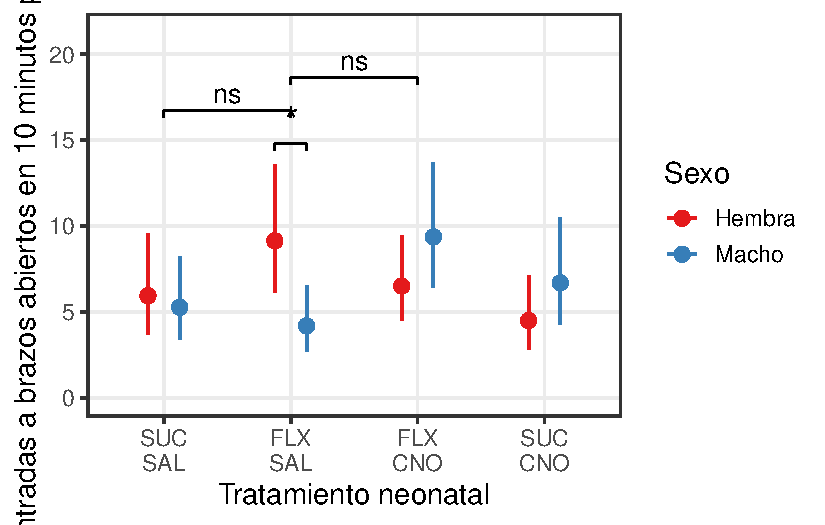
\includegraphics[keepaspectratio]{TP_Final_BIOME2_Informe_files/figure-pdf/gráfico final-1.pdf}}

}

\caption{\textbf{Figura 3.Entradas a brazos abiertos del laberinto en
cruz elevado (10 minutos) según tratamiento neonatal y sexo.} Los puntos
representan las medias estimadas por el modelo (binomial negativa mixto,
con camada como efecto aleatorio) y las barras, su intervalo de
confianza del 95 \%. Los corchetes indican los contrastes a priori, con
p ajustado por Bonferroni (3 contrastes): FLX vs SUC dentro de SAL
(promediando ambos sexos), CNO vs SAL dentro de FLX (promediando ambos
sexos) y hembras vs machos dentro de FLX SAL. * p \textless{} 0.05; ns,
no significativo. FLX: fluoxetina; SUC: sacarosa; CNO:
clozapina-N-óxido; SAL: salina.}

\end{figure}%

Como se ilustra en la Figura 3, las medias marginales estimadas para el
número de entradas a los brazos abiertos muestran un comportamiento
homogéneo entre la mayoría de las condiciones experimentales,
caracterizado por un amplio solapamiento de sus intervalos de confianza
del 95\%. Dicha amplitud refleja una marcada imprecisión en las
estimaciones puntuales, consecuencia de una elevada variabilidad
residual entre los individuos al interior de cada grupo experimental. La
diferencia más notable en la conducta exploratoria se concentra en el
grupo expuesto a fluoxetina sin inhibición prefrontal (FLX SAL), donde
las hembras exhiben una media estimada visiblemente superior y un
intervalo de confianza diferenciado del de los machos (p = 0.0116),
patrón que no se replica en los animales controles (SUC SAL) ni en los
tratados con CNO.

\subsection{Discusión}\label{discusiuxf3n}

El propósito de este estudio fue realizar inferencias a nivel
poblacional sobre el rol modulador de la corteza
prefro\textbf{Farji-Brener, A. G. (2003).} Uso correcto, parcial e
incorrecto de los términos hipótesis y predicciones en ecología.
Ecología Austral, 13(2), 223--227.

La prueba global de devianza indicó que la interacción triple entre los
factores no fue estadísticamente significativa (X\^{}2=1.30;p=0.2541).
Sin embargo, se detectó una interacción significativa entre la
inhibición quimiogenética prefrontal (generada por la administración de
CNO) y el sexo biológico (X\^{}2=10.43;p=0.0012). Este resultado
demuestra que el efecto de la desactivación de la CPF sobre la
exploración difiere sustancialmente entre machos y hembras. Dado que
ambas variables interactúan, sus efectos principales no deben
interpretarse de forma aislada, ya que respuestas de sentido opuesto
según el sexo ---un efecto de atenuación en machos frente a una
respuesta neutra o inversa en hembras--- se compensan mutuamente al
promediar.

Por su parte, el tratamiento neonatal con fluoxetina, al no participar
de interacciones significativas, permitió evaluar su efecto principal
poblacional, el cual no mostró diferencias significativas respecto al
vehículo (X\^{}2=1.74;p=0.187; Ratio=1.11;p=0.6836). Si bien la
literatura documenta que el exceso perinatal de serotonina altera el
refinamiento de las conexiones entre la CPF y el núcleo dorsal del rafe
(Teissier et al., 2017; Soiza-Reilly y Commons, 2011; Rayen et al.,
2011), la ausencia de significancia en la prueba principal no implica la
inexistencia del fenómeno biológico. Aunque no se podría descartar algún
problema de efectividad con la droga o el procedimiento experimental,
también podría indicar que una posible limitación de este estudio es el
tamaño reducido de réplicas para cada una de las combinaciones de los 3
factores, lo cual disminuye la potencia estadística para detectar
diferencias de magnitud pequeña. En consecuencia, las conclusiones que
se saquen de este estudio deben tomarse con cuidado, ya que existe una
probabilidad elevada de haber incurrido en Error Tipo II asociado a
limitaciones en la potencia estadística (Farji-Brener, 2003), es decir
que no se rechazan las hipótesis nulas (falso negativo).

Una posible explicación metodológica para esta falta de potencia
estadística radica en la estructura de varianza asociada al factor
camada. Al asignar las combinaciones de tratamientos a nivel de camadas
enteras, la variabilidad biológica, epigenética y del cuidado materno
entre camadas pudo haber actuado como una fuente considerable de ruido
residual. De acuerdo con diversos estudios neurotoxicológicos y
comportamentales en roedores, la varianza atribuible al efecto de camada
puede llegar a representar habitualmente entre un 30\% y un 60\% de la
variabilidad total observada en pruebas conductuales (Houwing et al.,
2019; Sobin et al., 2019). Frente a este escenario, la literatura
metodológica sugiere que la implementación de diseños en bloques
completos dentro de cada camada (litter-matched controls) constituye una
alternativa eficaz para reducir el error residual, al permitir extraer
la variancia compartida entre camadas y optimizar la capacidad de
detectar el efecto de los tratamientos. Sin embargo, dada la limitación
biológica en el tamaño de camada característico de la cepa C57BL/6, la
conformación de bloques intra-camada completos con representación de
todas las combinaciones de tratamientos y sexos resultaría difícil de
alcanzar en la práctica. Por lo tanto, en futuros ensayos se sugiere
evaluar el empleo de cepas con mayor prolificidad y camadas más
numerosas que faciliten la viabilidad técnica de este esquema de
bloqueo.

A pesar de estas limitaciones, el estudio aportó evidencia concluyente a
favor de la Hipótesis 3, demostrando una marcada resiliencia diferencial
por sexo en animales expuestos a fluoxetina sin inhibición prefrontal
(Ratio=2.18; IC 95\%: {[}1.28;3.69{]}; p=0.0039). A nivel poblacional,
las hembras tratadas con fluoxetina registran una esperanza de entradas
a brazos abiertos 1,18 veces mayor que los machos bajo la misma
condición. Este resultado respalda la noción de que el cerebro femenino
posee mecanismos endógenos de protección frente a perturbaciones
serotoninérgicas tempranas (Houwing et al., 2019; Rayen et al., 2011).~

En conclusión, la respuesta a la modulación quimiogenética de la CPF
frente a la elevación neonatal de serotonina se encuentra
intrínsecamente condicionada por el sexo biológico. Aunque la dispersión
entre camadas limitó la potencia para detectar el efecto principal de la
fluoxetina a nivel global, la confirmación de la mayor resiliencia en
hembras y la interacción de la inhibición prefrontal con el sexo aportan
hallazgos neurobiológicos clave, destacando la necesidad de adoptar
diseños experimentales bloqueados por camada en futuras investigaciones.

\subsection{Bibliografía}\label{bibliografuxeda}

\begin{itemize}
\item
  \textbf{Farji-Brener, A. G. (2003).} Uso correcto, parcial e
  incorrecto de los términos hipótesis y predicciones en ecología.
  Ecología Austral, 13(2), 223--227.
\item
  \textbf{Gallo, M. T., Virenque, A., Golinelli, A., Fumagalli, F.,
  Castrén, E., Brivio, P., \& Calabrese, F. (2025).} From early-life
  fluoxetine exposure to lifelong, sex-specific behavioral changes:
  decoding the dynamics of sensitive periods. Molecular Psychiatry, 31,
  1205--1215. https://doi.org/10.1038/s41380-025-03223-6
\item
  \textbf{Houwing, D. J., Staal, L., Swart, J. M., Ramsteijn, A. S.,
  Wöhr, M., de Boer, S. F., \& Olivier, J. D. A. (2019).} Subjecting
  dams to early life stress and perinatal fluoxetine treatment
  differentially alters social behavior in young and adult rat
  offspring. Frontiers in Neuroscience, 13, 229.
\item
  \textbf{Rayen, I., van den Hove, D. L., Prickaerts, J., Steinbusch, H.
  W., \& Pawluski, J. L. (2011).} Fluoxetine during development reverses
  the effects of prenatal stress on depressive-like behavior and
  hippocampal neurogenesis in adolescence. PLoS ONE, 6(9), e24003.~
\item
  \textbf{Sobin, C., et al.~(2019).} Statistical modeling with litter as
  a random effect in mixed models. Neurotoxicology and Teratology, 77,
  106841.~
\item
  \textbf{Soiza-Reilly, M., \& Commons, K. G. (2011).} Glutamatergic
  drive of the dorsal raphe nucleus. Journal of Chemical Neuroanatomy,
  41(4), 247--255.
\item
  \textbf{Soiza-Reilly, M., \& Commons, K. G. (2014).} Unraveling the
  architecture of the dorsal raphe synaptic neuropil using
  high-resolution neuroanatomy. Frontiers in Neural Circuits, 8, 105.
\end{itemize}




\end{document}
